\chapter{Trajectory Replanning for Obstacle Avoidance}%
\label{CH:AVOIDANCE}

%----------------------------------------------------------------------------------------
\section{The Framework}
React to the unknown, avoid previously unseen obstacles, and replan trajectories in real-time are three basics capabilities
that take part inside the set of elementary abilities that an autonomous robot must master before being able to start moving in
real-world environments, cluttered of objects, people, animals, cars, and hopefully other robots, which may behave unpredictably.
Due to the importance of the problem at hand, a huge number of solutions have been presented in the literature, first in a pure
path planning approach~\cite{mehdi2015collision}, where the timing law is not considered during the planning stage and its computation
is left as a posteriori task, later in a direct trajectory planning framework~\cite{ding2019efficient}, where the path and timing law
are concurrently computed, letting the planner to exploit the full robot capabilities and to shape the path in order to ease the
time allocation for a final feasible trajectory. Although we saw very impressive works in this field, very few of them try to
approach the planning, or replanning, problem from a numeric point of view, and even fewer try to use consolidated control system
theory to guarantee the convergence of the planning algorithm. It results that, although the proposed solutions work well in 
simulations, or in not-too-complex environments, their failure rate in real environments is very high. Besides that, careful
parameters tuning is often required, yielding to a very poor generalization. With the aforementioned problems in mind, we try to
contribute by firstly analyzing, and implementing on our flight platform, a carefully selected state-of-the-art replanning algorithm,
to test its performance in real-world scenarios, then we try to perturb the current trend of purely algorithmic solutions
by proposing two numerical and control-oriented approaches.
In this chapter, we aim to review three different avoidance techniques starting from a purely algorithmic solution, borrowed from
the state of the art, to more numerical and control-oriented ones, which instead represent original unpublished works.
The core concept behind the proposed solutions is represented by the idea that treating the problem of obstacle avoidance numerically
allows assessing its performances via stability analysis tools, borrowed from the control theory field, which ensures convergence in
all cases where some conditions are fulfilled, unlike purely algorithmic approaches where the convergence to a correct solution is not
guaranteed at all. Although the reader hardly finds in this thesis the aforementioned stability analysis, the algorithm presentation, as well
as the research carried out in this field, is oriented in this direction.

\subsection{Related Works}
The trajectory replanning framework is a large field of study that may embrace several different solutions, often quite variegated
with different inputs and outputs, and suitable for different environmental conditions where only static obstacles are present,
where moving objects may suddenly appear, or where other robotic agents move, with the possibility to networking and share motion
information. Due to this variety, the referring literature is as large as to be unmanageable, even focusing on a specific problem,
so we choose to mention here the most important works which motivated this thesis more. In particular, we first focused on the problem
of static obstacles avoidance, then moved to the case with moving objects, overlooking the multi-agent case, being that a specialization
of the more general one where objects move with a priori unknown pattern.
In this field, the first sharp split in the research direction was caused by the introduction of the B\acuteacc ezier curves as a new trajectory
parameterisation approach, pioneer of this idea was~\cite{choe2015trajectory}, where this parameterisation was used to plan fixed-wing aircraft
trajectories. The good properties of such curves allowed for easy arc length computation and collision checking, thanks to which the approaches
developed with this tool outperform classical solutions based on polynomial trajectories~\cite{oleynikova2016continuous, richter2016polynomial}.
The work~\cite{choe2015trajectory} introduced also a novel concept of time allocation as curve composition, allowing to use the same curve properties
not only for spatial paths but also to shape the associated timing law. This innovative idea dropped into obsolescence due
to the complexity of evaluating high-order derivatives. As a matter of fact, further works in this field, which exploit the B\acuteacc ezier curves
properties, were devoted only to modifying the current agent path, ensuring dynamic continuity, but without keeping into account the possibility of
locally changing the allocated timing law~\cite{mehdi2015collision, mehdi2019collision}.
B\acuteacc ezier curves were subsequently used in an uncountable number of works, together with their strict brother, the B-splines.
The work of~\cite{gao2019flying} proposes to use B\acuteacc ezier curves to plan trajectories inside the pointclouds retrieved from LiDAR
sensor updates, while~\cite{zhou2021raptor} makes use of B-splines to ensure trajectory feasibility during optimisation.
The works of ~\cite{park2022online} and~\cite{park2020efficient} exploit the convex hull containments property to avoid collisions, constraining the planned curve inside a set
of convex safe corridors iteratively updated in time, while~\cite{tordesillas2021mader} used B-splines to represent both robot and
obstacle dynamics, a carefully selected and optimized set of separation planes was used to keep the planned path safe.
A new recent trend was finally introduced by~\cite{ding2019efficient}, who first proposed a novel sampling-based approach meant for
directly planning B-spline trajectories. The basic idea was to translate the classic robot pose sampling, into a higher dimensional space
where each sample configuration represents directly a piece of possible trajectory, allowing for dynamical considerations.
Although some state-of-the-art works may consider time allocation as an active part of the problem at hand~\cite{ding2019efficient, park2020efficient, tordesillas2021mader}
there is no explicit optimization procedure that allows its computation yet, losing a set of degrees of freedom especially useful in highly cluttered environments.
Besides the approaches just analyzed, which consider a time-parameterised trajectory as algorithm output, there exist other solutions
that try to elevate the problem abstractness to a higher level, considering velocity, or acceleration, as algorithm output, allowing for
easier control algorithms at the plant side.
In this field, it is worth mentioning the works of~\cite{cieslewski2017rapid} and~\cite{falanga2020dynamic} which select the robot velocity
on the basis of a reconstructed map of the environment in the former case, and on the basis of event camera updates in the latter one.
Furthermore, learning-based techniques obtained impressive results when trained to compute safe velocity commands~\cite{loquercio2018dronet, loquercio2021learning}.
Finally, other approaches take into consideration the full robot dynamics via model predictive control~\cite{penin2018vision}, or
control barrier functions~\cite{wang2017safety, singletary2021comparative, khan2022gaussian} solutions.
The latters, although more complicated, allow the use of control system tools to verify stability, ensuring convergence to a feasible solution
under a set of well-specified assumptions.

\subsection{Problem Definition}%
\label{SEC:REPLANNING-PROBLEM-DEFINITION}
The problem of trajectory replanning is strictly linked to the problem of planning, with the only difference that, in the former case,
is supposed a prior notion of a dynamically feasible trajectory, which may become unfeasible due to possible collisions when new
sensor readings become available. Let $\lp \xx \lp t \rp, \uu \lp t \rp \rp$ be an initial feasible state trajectory, solution of 
\begin{equation*}
    \dot{\xx} = \xfun \lp \xx, \uu \rp,
\end{equation*}
and satisfying $\xx \in \xset$ and $\uu \in \uset$. Where $\xfun \lp \cdot \rp$ represents the robot dynamics, while $\xset \in \R^{\dd{\xx}}$
and $\uset \in \R^{\dd{\uu}}$ are the allowed sets for $\xx$ and $\uu$, respectively. Then the problem of replanning can be formalized as the
computation of the tuple $\lp \xx\s \lp t \rp, \uu\s \lp t \rp \rp$ as a solution of the optimisation problem
\begin{equation}%
    \label{EQ:REPLANNING-OPTIMISATION-PROBLEM}
    \begin{split}
        \min_{\xx', \uu'} & \norm{\xx - \xx'} + \norm{\uu - \uu'}, \\
        \text{subj. to} \hspace{0.3cm} & \xx' \in \xset', \hspace{0.3cm} \uu' \in \uset', \\
        & \dot{\xx}' = \xfun \lp \xx', \uu' \rp,
    \end{split}
\end{equation}
with $\xset'$ and $\uset'$ the new allowed sets computed after the integration of the new sensor readings.
Note that~\eqref{EQ:REPLANNING-OPTIMISATION-PROBLEM} addresses the problem of replanning by looking for a new feasible trajectory
that lies as close as possible to the original one. This choice is motivated by the idea that if an initial trajectory was provided, it
was optimal for the task at hand, and computed by minimising a precise index.
Although problem~\eqref{EQ:REPLANNING-OPTIMISATION-PROBLEM} embraces a large number of use cases addressed in the literature, it misses the
case where the safe set $\xset$ is not fixed in time, thus in the environment are present moving objects, or other agents.
In this view, let us suppose to have the knowledge of how these objects, or agents, move, having at hand an estimation of their current
trajectory in terms of $\rr_o = \lp x_o, y_o, z_o \rp$ position. Moreover, let $\Gamma \lp \xx \rp$ the map able to extract, from the
current state trajectory, only the $x,y,z$ components expressing the agent position in space. Thus problem~\eqref{EQ:REPLANNING-OPTIMISATION-PROBLEM}
can be rewritten as
\begin{equation*}
    \begin{split}
        \min_{\xx', \uu'} & \norm{\xx - \xx'} + \norm{\uu - \uu'}, \\
        \text{subj. to} \hspace{0.3cm} & \xx' \in \xset', \hspace{0.3cm} \uu' \in \uset', \\
        & \dot{\xx}' = \xfun \lp \xx', \uu' \rp, \\
        & \norm{\Gamma \lp \xx \lp t \rp \rp - \rr_o \lp t \rp} > d_{\text{safe}} \hspace{0.3cm} \forall t \in \R_{+},
    \end{split}
\end{equation*}
with $d_{\text{safe}} \in \R_{\ge 0}$ expressing the minimum distance intra-agent, or between the considered agent and the moving obstacle.
In the particular case of a quadcopter, its differential flatness property allows to ease the optimisation procedure by directly
optimise on the space of its flat outputs $\flatoutput =  \lp x, y, z, \yaw \rp = \lp \rr, \yaw \rp$.
For more details about this property please refer to~\secref{SEC:DIFFERENTIAL-FLATNESS}.

%----------------------------------------------------------------------------------------
\section{On Flight Trajectory Replanning}%
\label{SEC:REPLANNING-ALGORITHM}
In this section we review and adapt a purely algorithm solution to the problem stated in~\secref{SEC:REPLANNING-PROBLEM-DEFINITION},
in particular we focused on the solution proposed by~\cite{zhou2021raptor} being the state-of-the-art work that shows the most
promising results. We borrowed from~\cite{zhou2021raptor} the core idea, while the algorithm implementation, as well as its integration
inside our operative framework has been completely developed internally. The reviewed solution has been successfully coupled with a
fast and reliable perception stack, that allows to detect possible collisions and triggers the replanning system, as well as the control
layer. Moreover, we proposed a novel solution, exploiting the B-spline properties, to fast link the replanned trajectory with
the previously provided one, ensuring continuity up to the adopted spline order. Experimental results show how the proposed stack is
effective in fast replanning colliding trajectories, and how continuity is always guaranteed.

The proposed replanning system takes the outputs of a global planning procedure,
along with the perception, or mapping, output, and the current robot position, and deforms the global reference trajectory locally
to avoid previously unknown obstacles. The replanning works in two steps. Firstly, a set of local guiding paths are generated through
the free space, although may there exists an infinite number of possible paths we restrict the final choice only to those dinstictive paths
considered as \emph{topologically different}, by pruning the ones bringing more detour from the initial planned trajectory.
Secondly, a B-spline-based Path-Guided Optimisation (GTO) step is in charge to build a set of locally optimal trajectories out from the
found paths. The \quotopen best\quotclosed trajectory is then extracted and executed.

\subsection{Collision Perception \& Replanning Trigger}
In order to check the trajectory safeness, we employ two different data structures (a) an Euclidean Signed Distance Field (ESDF), which
is in charge to represent the known environment obstacles, and is continuously updated with new sensor readings, and (b) a ktree structure
built on the last pointcloud computed via stereo image matching. The necessity to employ two different data structures may seem as an
useless redundancy, since them are actually representing the same information, but is of fundamental importance to maintain the time consistency of
the data. As a matter of fact, the integration of new measurements inside any map structure is costly and cannot be made completely real-time, 
moreover checking the current trajectory in the sensor frame may improve the solution robustness against position estimation errors and
sensor noise. The same structures are then later used to generate the topological paths, and to steer the path-guided optimisation away
from the detected obstacles.
The perception layer works by continuously checking, at each new sensor reading, the currently running trajectory for possible collisions
inside both the current pointcloud, via ktree nearest search, and inside the current reconstructed ESDF. In particular,
the running trajectory is checked for collisions in a sliding time window of fixed-dimension $T_{\text{max}}$, at a fixed resolution
of $\Delta_T$. The initial time of the window is chosen in order to correspond exactly to the current robot position, while $T_{\text{max}}$
results from a tradeoff between algorithm performances, sensor range, and the robot capabilities.
If a collision is detected very close to the current position, let's say there exists a minimum allowed time $t_{\text{min}}$, then an
emergency stop procedure is triggered, and the robot tries to apply all efforts in slowing down and stop as fast as possible.
On the other hand, if a collision is detected on a feasible time, the replanning procedure is triggered.
In order to let the solution be resilient versus sensor noise and false detections, we inject a lower bound $N_{\min}$ of consecutive detections
before considering the current trajectory unsafe.

\subsection{Topological Path Searching}
The core of the proposed solution is a Gradient-based Trajectory Optimisation (GTO) which allows to formulate locally optimal and safe trajectories in real-time.
GTO methods, which typically formulate trajectory generation as non-linear optimization problems, trading off smoothness, safety and dynamic feasibility, are shown
to be particularly effective in local replanning~\cite{zhou2020robust, oleynikova2016continuous, gao2017gradient, usenko2017real}, but
previous works~\cite{schulman2014motion} showed that GTO methods are very sensitive to unfavorable initialization, which may even lead to 
unfeasible solutions. Typical GTO methods incorporate the gradients of a ESDF in a collision cost to push the trajectory out of obstacles.
Yet there are some \quotopen valleys\quotclosed or \quotopen ridges\quotclosed in the ESDF, around which the gradients differ greatly.
Consequently, if a trajectory is in collision and crosses such regions, the gradients of ESDF will change abruptly at some points.
This can make gradients of the collision cost push different parts of the trajectory in opposing directions and fail the optimisation.
Normally, such points, which correspond to the space that has an identical distance to the surfaces of nearby obstacles,
are difficult to avoid, especially in complex environments. Therefore, optimization depending solely on the ESDF fails inevitably at times.
To solve the problem, it is essential to introduce extra information that can produce an objective function whose gradients consistently
deform the trajectory to the free space. For this reason, we adopt a sampling-based topological path searching to find a collection of
distinctive paths, later used inside the proposed GTO method reformulated as a GPO.

Whereas there exists an infinite number of possible paths, we restrict the GPO procedure to apply to a subset of distinctive paths, that
are considered topologically different. In this sense, we employ the notion of \emph{Uniform Visibility Deformation} (UVD) firstly introduced in~\cite{zhou2021raptor},
which provides a constructive method to assess the sampled paths equivalency.
\begin{definition}
    Two trajectories $\spline_1 \lp \splinevar \rp$, $\spline_2 \lp \splinevar \rp$ parameterized by $\splinevar \in \lps 0,1 \rps$ and satisfying
    $\spline_1 \lp 0 \rp = \spline_2 \lp 0 \rp$, $\spline_1 \lp 1 \rp = \spline_2 \lp 1 \rp$, belong to the same uniform visibility deformation class,
    if for all $\splinevar$, the line $\overline{\spline_1 \lp \splinevar \rp \spline_2 \lp \splinevar \rp}$ is collision-free.
\end{definition}
The proposed solution works by building a roadmap capturing an abundant set of paths from different UVD classes.
Unlike standard roadmap planning algorithms, which create maps containing many redundant loops, the adopted method generates a more
compact roadmap where each UVD class contains just one or a few paths.
The final roadmap is iteratively created as a graph connecting a series of nodes, randomly sampled in the $x,y,z$ configuration space.
Each sampled node can be recognised as a \emph{guard} or a \emph{connector}. Guards are responsible for exploring different parts of the
free space, while connectors connect two guards to create a feasible piece of path.
Any two guards $g_1 \in \R^3$ and $g_2 \in \R^3$ of the graph cannot be visible to each other, i.e. the line $\overline{g_1 g_2}$ is in collision,
thus every time a sampled point is invisible to all other guards, a new guard is created. On the other hand, if a sampled point is visible at least from
two guards, a new connector is created and all possible paths, connecting the latter node to all visible guards, are generated.
Finally, if a sampled node is visible from only one guard is discarded.
The newly generated paths are added to the global roadmap only if belong to a different UVD class, or the counterpart of the same class
represents a longer path.
In the beginning, the roadmap graph is initialized with exactly two guards, representing the starting and goal points.
The start position is computed as the point corresponding to half of the detected collision time $t_{\text{coll}}$
(i.e. $t_{\text{start}} = 0.5t_{\text{coll}}$), while the goal is selected as the point far at least $d_{\text{obs}}$ from the
detected collision point, at time $t_{\text{goal}}$. In this setting, halving the collision time turns out to be effective to
instantiate enough time for the replanning procedure, while the robot is moving, and $d_{\text{obs}}$ is provided as an input
parameter. We stress the fact that $d_{\text{obs}}$ is representative of a priori notion about the surrounding environment,
being it ideally the maximum obstacle size that the robot should avoid. A wrong tuning of $d_{\text{obs}}$ may lead to further
unnecessary replanning procedure, which may even fail if the guessed value is too far from the real one. The graph growth continues
until a limit of time $\Delta_{\text{max}}$ of a limit of sampling nodes $N_{\text{max}}$ is reached. With the roadmap at hand,
a depth-first search algorithm, augmented by a visited node list, is applied to search for all the possible paths between the
start and goal node, in a similar way as done in~\cite{rosmann2017integrated}.

\subsection{Path Shortening and Optimisation}%
\label{SEC:REPLANNING-OPTIMISATION}
The extracted paths may present two distinctive pathologies, on the first stage they may present very high detours from the original trajectories,
and in the second stage may be redundant in the UVD sense, even if redundant connections between two guards are avoided.
In order to correct these unwanted pathologies, we firstly search for topologically equivalent shortcut path for each one, then
we check the equivalence between any two paths and only preserve topologically distinct ones.
In particular, to perform shortening, each found path is discretised with a fixed resolution $d_{\text{res}}$ and a new path
is generated by adding the discretised points, one to each other, only if the considered point is not visible from the last added point.
The aforementioned procedure generates shorter, but infeasible, paths, due to not visibility condition.
To solve this problem, all infeasible points of the new paths are pushed away from obstacles in the direction of the ESDF gradient, of
a fixed distance $d_{\text{safe}}$. Then the generated paths are checked for equivalence to preserve only topologically distinct ones.
It is worth to remark that the number of distinctive paths grows exponentially with the number of obstacles, and in case of complex environments,
it is computationally intractable to use all paths. For this reason, we only select the first $N_{\text{paths}}$ shortest paths.

Once a set of topologically different short paths, connecting the start and goal node, have been collected, a PGO procedure is employed to
optimise all found paths and allocate a feasible timing law. The optimisation procedure is efficiently performed using B-spline parameterisation and
by parallelizing the computation load on all available cores.
The proposed PGO method follows a two steps approach, the first phase is devoted to generate a \emph{warmup trajectory} by deforming the
current one toward the selected path, that lies on the free and flyable space. While, in the second phase the obtained solution is
iteratively refined via nonlinear optimisation to push it away from obstacles and to guarantee its dynamical feasibility.
Going down in the details, the trajectory segment in collision is reparameterized as a $\order$-degree B-spline $\spline \lp \splinevar \rp$
with control points $\CP = \lps \bs{\cpoint}_0, \dots, \bs{\cpoint}_{\cpnumber} \rps$ and knot vector
\begin{equation*}
	\bs{\splinevar} =
	\begin{bmatrix}
		0_{0:\order}, & \Delta_{\splinevar}, & 2\Delta_{\splinevar}, & \dots, & (\cpnumber-\order)\Delta_{\splinevar}, & T_{0:\order}
	\end{bmatrix},
\end{equation*}
where $\cpnumber$ is given by the chosen discretisation resolution $d_{\text{res}}$, while $T$ correspond with the time elapsed from
the selected initial to the goal point. In this setting, the first phase correspond to the solution of the following optimisation problem
\begin{equation}%
    \label{EQ:REPLANNING-FIRST-PHASE}
	\min_{\bs{\cpoint}_{0}, \dots, \bs{\cpoint}_{\cpnumber}}
				\lambda_1 \int_0^{T} \norm{\frac{d^3 \bs{\spline} \lp \splinevar \rp}{d \splinevar^3}}^2 d \splinevar
				+ \lambda_2 \sum_{i=0}^{\cpnumber} \norm{\bs{\cpoint}_i - \rr_i}^2,
\end{equation}
with $\lambda_1, \lambda_2 \in \R_+$, and $\rr_i$ with $i = 0, \dots, \cpnumber$ represents the discretised points obtained from the 
collected topological paths. In problem~\eqref{EQ:REPLANNING-FIRST-PHASE}, the first loss term aims to improve the final trajectory
smoothness, while the second one penalizes its distance from the guiding path. Both the terms can be simplified in their formulation using
the B-spline properties (\secref{SEC:SPLINES-APPENDIX}), yielding to an unconstrained quadratic programming problem, that can be
easily solved in closed form. The first phase outputs a smooth trajectory in the vicinity of the guiding path.
Since the path is already collision-free, usually the warmup trajectory is also so. Even though it is not completely collision-free,
its major part will be attracted to the free space. At this stage, the gradients of ESDF along the trajectory vary smoothly,
and the gradients of the objective function push the trajectory to the free space in consistent directions.
In the second phase, we adopt a nonlinear optimisation framework to further refine the warmup trajectory into a smooth, safe,
and dynamically feasible one.
\begin{equation}%
	\label{EQ:REPLANNING-SECOND-PHASE}
	\begin{split}
	\min_{\bs{\cpoint}_{0}, \dots, \bs{\cpoint}_{\cpnumber}} &
				\lambda_1 \int_0^{T} \norm{\frac{d^3 \bs{\spline} \lp \splinevar \rp}{d \splinevar^3}}^2 d \splinevar
				+ \lambda_2 \sum_{i=0}^{\cpnumber} \mathcal{F} \lp \bs{\cpoint}, d_{\text{safe}}\rp, \\
	\text{sub.to.} \hspace{0.3cm} &
				\bs{\cpoint}_i' \le v_{\text{max}} \hspace{0.3cm} \forall i = 0, \dots, \cpnumber-1, \\
				& \bs{\cpoint}_i'' \le a_{\text{max}} \hspace{0.3cm} \forall i = 0, \dots, \cpnumber-2, \\
				& \bs{\cpoint}_0 = \rr_0, \hspace{0.3cm} \bs{\cpoint}_{\cpnumber} = \rr_{\cpnumber}, \\
				& \bs{\cpoint}_0' = v_{\text{init}}, \hspace{0.3cm} \bs{\cpoint}_0'' = a_{\text{init}},
	\end{split}
\end{equation}
where $\mathcal{F} \lp \bs{\cpoint}, d_{\text{safe}} \rp$ shapes as
\begin{equation*}
    \mathcal{F} \lp \bs{\cpoint}, d_{\text{safe}} \rp =
    \begin{cases}
        0 & \text{if } d \lp \bs{\cpoint} \rp \ge d_{\text{safe}}, \\
        \lp d \lp \bs{\cpoint} \rp - d_{\text{safe}} \rp^2 & \text{if } d \lp \bs{\cpoint} \rp < d_{\text{safe}}.
    \end{cases}
\end{equation*}
In the aforementioned equation, $d \lp \bs{\cpoint} \rp$ is the distance of $\bs{\cpoint}$ from the closest obstacle evaluated using both
the ESDF map and the ktree built out of the current sensor reading.
Once all topological paths as been time parameterised and optimised, the trajectory leading to the minimum cost is extracted and executed.
Although the proposed PGO has one more step of optimization compared with previous methods, it can generate better trajectories within
shorter time. The first-phase takes only negligible time, but generate a warmup trajectory that is easier to be further refined,
which improve the overall efficiency.

\subsection{B-Spline Trajectory Injection}
%%%%%%%%%%
\begin{figure}[!t]
	\begin{center}
		\begin{minipage}{.45\linewidth}
			\centering
			\subfloat[]{%
				\label{FIG:REPLANNING-RESULTS-TRAJECTORY-A}%
				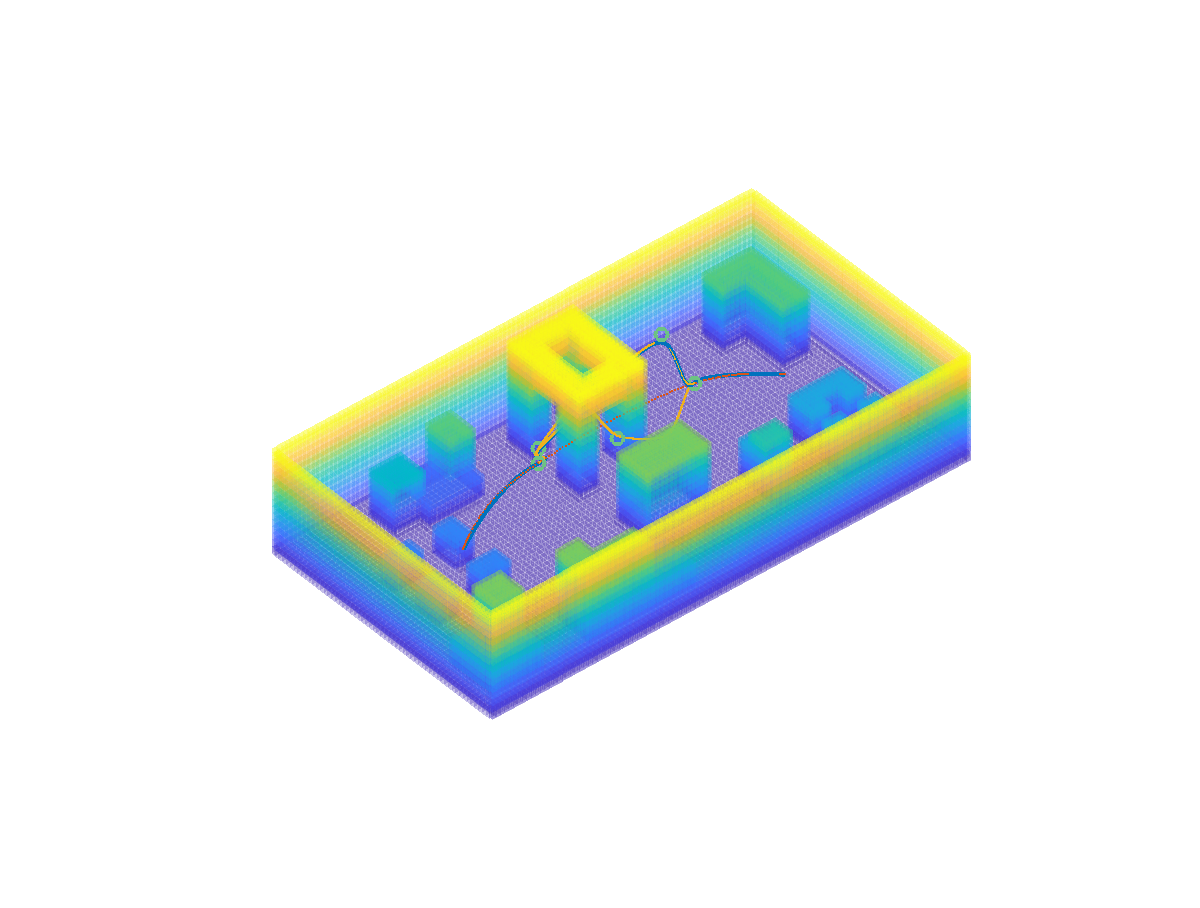
\includegraphics[trim={3.5cm 2.5cm 3cm 2.5cm}, clip = true, width = 1.05\textwidth]{Figs/Chapter6/replan_3d_traj_1.eps}}
		\end{minipage}
		\begin{minipage}{.45\linewidth}
			\centering
			\subfloat[]{%
				\label{FIG:REPLANNING-RESULTS-TRAJECTORY-B}%
				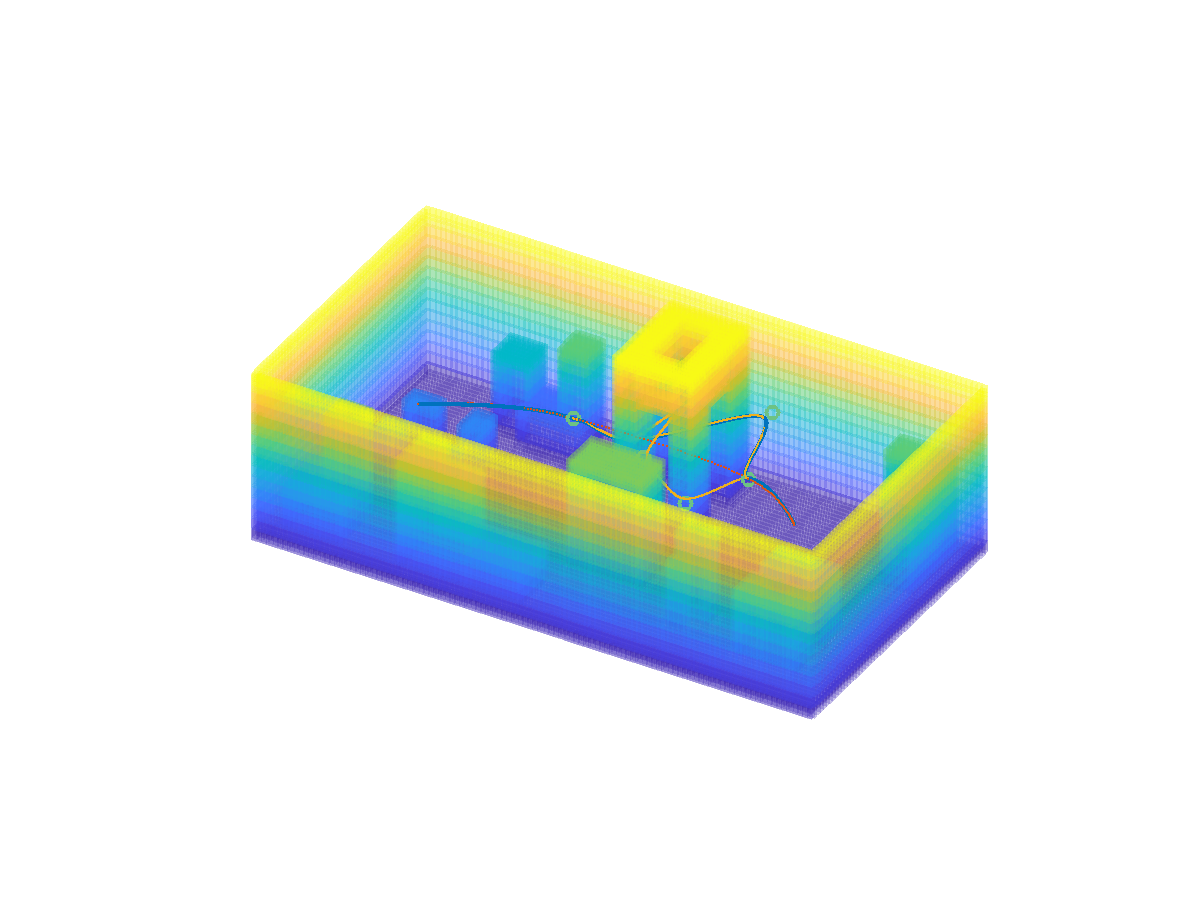
\includegraphics[trim={3.5cm 2.5cm 3cm 2.5cm}, clip = true, width = 1.05\textwidth]{Figs/Chapter6/replan_3d_traj.eps}}
		\end{minipage}
	\end{center}
	\caption{Results of the reviewed approach in the synthetic environment adopted in the Leonardo drone contest.
    The solution was able to replan feasible and safe trajectories in real-time, without forcing the quadcopter to an emergency stop.
    In the figure, the red path represents the initial colliding trajectory, the yellow points are the optimised hypothesis for replanned
    trajectory, and the blue path represents the final choice. Images (a) and (b) depict the same simulation, captured from two different
    points of view.}%
    \label{FIG:REPLANNING-RESULTS-TRAJECTORY}
\end{figure}
%%%%%%%%%%
The optimisation problem~\eqref{EQ:REPLANNING-SECOND-PHASE} yields to locally optimal trajectories guaranteed to be continuous up to
the second derivative, with the initial colliding trajectory. This is a fundamental feature since the tree segments, namely the first initial
trajectory, the replanned piece, and the final one, must be executed one after each other, consecutively.
Some issues may arise when the replanning procedure is called several times, during the execution of a previously replanned segment.
Indeed, the replanner may commission an even large number of trajectory pieces, that quickly become intractable for the reference generator.
Moreover, if the application at hand requires a higher level of continuity, this new requirement must be encoded inside~\eqref{EQ:REPLANNING-SECOND-PHASE}
which at the end may take too much time to solve.
In this section we propose a novel method to join the new replanned segment with a previously computed B-spline trajectory.
The proposed method is as simple as effective, it ensures continuity up to the spline order and outputs only one trajectory,
allowing for any replanning procedure as required by the surrounding environment.
The key idea comes from the B-spline property to be shaped, at each time instant $\splinevar \in \lps 0, T \rps$, by only $\order+1$
control points. It follows that, splitting the control points vector exactly in the correspondence of the final $(\order+1)$th control point
that spans the curve at time $t_{\text{start}}$ and the first control point that spans the curve at $t_{\text{goal}}$, allows for
inserting the new set of points, identifing the replanned curve, without loosing any spline continuity feature.
Finding the splitting points can be easily done by checking the knot span for the first $u_i \ge t_{\text{start}}$ and 
$u_j \ge t_{\text{goal}}$, then converting the found value in terms of the corresponding control point indeces $i_{\text{cp}}$
and $j_{\text{cp}}$ as
\begin{equation*}
    \begin{split}
        i_{\text{cp}} & = i - \left \lceil \order/2 \right \rceil - 2, \\
        j_{\text{cp}} & = j - \left \lceil \order/2 \right \rceil - 1. \\
    \end{split}
\end{equation*}
Giving two control points sequences $\CP^1 = \lps \bs{\cpoint}^1_0, \dots, \bs{\cpoint}^1_{\cpnumber^1} \rps$ and
$\CP^2 = \lps \bs{\cpoint}^2_0, \dots, \bs{\cpoint}^2_{\cpnumber^2} \rps$, with the corresponding knot vectors
$\bs{\splinevar}^1 = \Big[ 0_{0:\order}, \Delta^1_{\splinevar}, \dots,$ $(\cpnumber^1-\order)\Delta^1_{\splinevar}, T^1_{0:\order} \Big]$
and $\bs{\splinevar}^2 = \lps 0_{0:\order}, \Delta^2_{\splinevar}, \dots, (\cpnumber^2-\order)\Delta^2_{\splinevar}, T^2_{0:\order} \rps$,
representing the initial and replanned trajectory respectively, then the composed curve with control points
\begin{equation*}
    \CP = \lps \bs{\cpoint}^1_0, \dots, \bs{\cpoint}^1_{i_{\text{cp}}}, \bs{\cpoint}^2_0, \dots, \bs{\cpoint}^2_{\cpnumber^2}, \bs{\cpoint}^1_{j_{\text{cp}}}, \dots, \bs{\cpoint}^1_{\cpnumber^1} \rps,
\end{equation*}
and knot vector
\begin{equation*}
    \bs{\splinevar} =
    \begin{bmatrix}
        0_{0:\order}, & \Delta^1_{\splinevar}, & 2\Delta^1_{\splinevar}, & \dots, & ((\cpnumber^2 + \cpnumber^1 - j_{\text{cp}} + i_{\text{cp}}) - \order)\Delta^1_{\splinevar}, & T_{0:\order}
    \end{bmatrix},
\end{equation*}
preserves the path described by the consecution of the aforementioned three segments, ensuring continuity up to the chosen spline order.

\subsection{Experimental Results}
%%%%%%%%%%
\begin{figure}[!t]
	\begin{center}
		\begin{minipage}{.45\linewidth}
			\centering
			\subfloat[]{%
				\label{FIG:REPLANNING-RESULTS-VELOCITY-A}%
				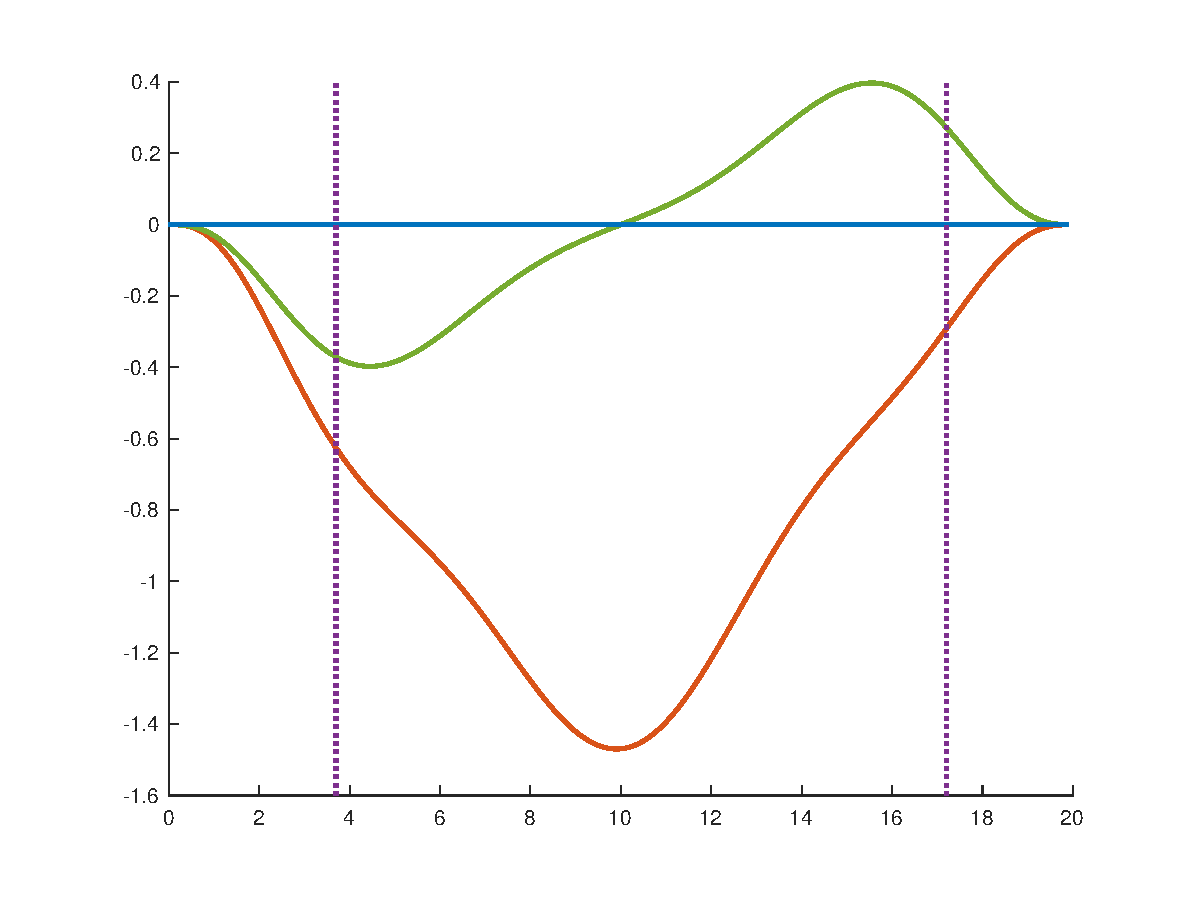
\includegraphics[width = 1.05\textwidth]{Figs/Chapter6/replan_init_vel.eps}}
		\end{minipage}
		\begin{minipage}{.45\linewidth}
			\centering
			\subfloat[]{%
				\label{FIG:REPLANNING-RESULTS-VELOCITY-B}%
				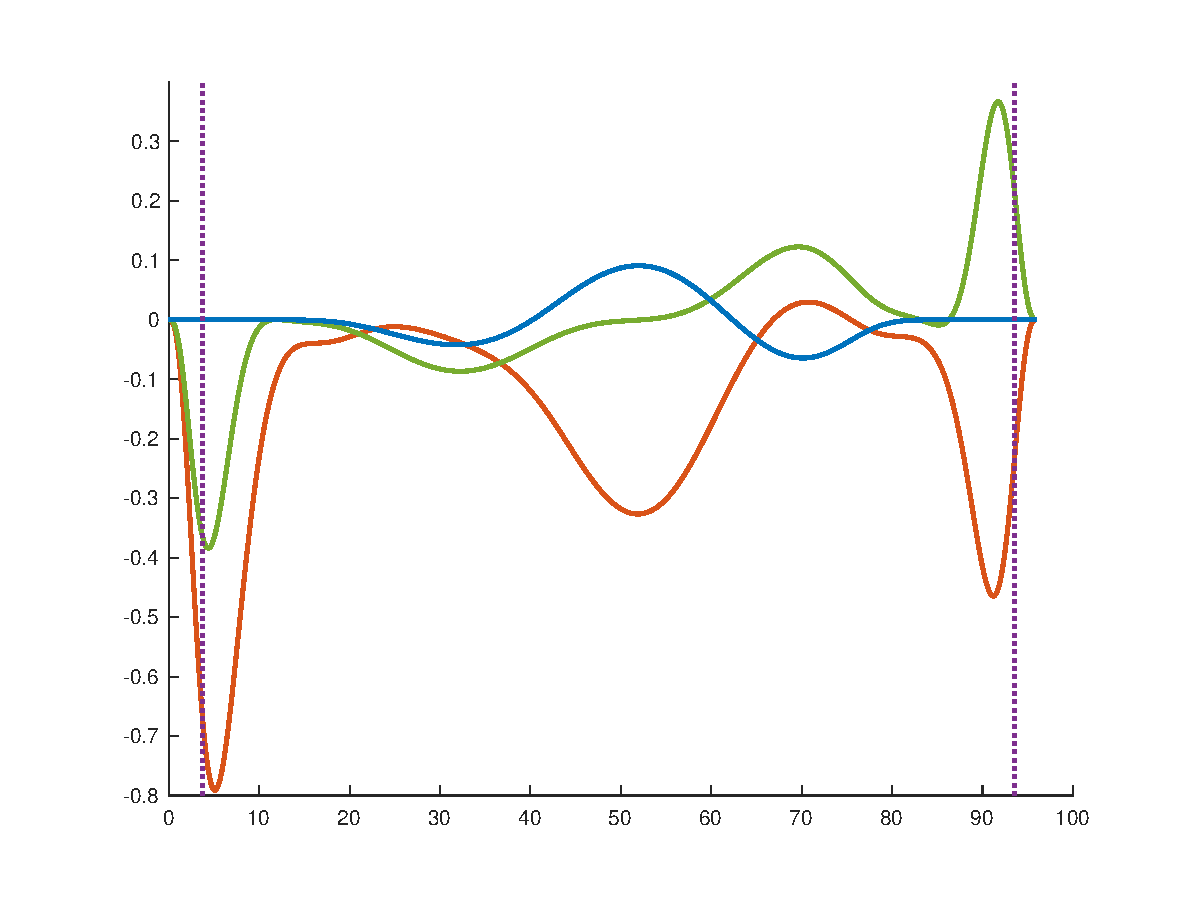
\includegraphics[width = 1.05\textwidth]{Figs/Chapter6/replan_post_vel.eps}}
		\end{minipage}
	\end{center}
	\caption{Initial velocity trajectory (a) and replanned one (b).
    In the images, the red line represents the velocity along the x-axis, the green one is the velocity along the y-axis,
    and the blue represents the velocity along the z-axis. The two vertical purple lines mark the initial and final cutting
    points, where the initial trajectory is broken and reconnected with the replanned one. Note that the velocity continuity
    is completely preserved. In both cases the velocity is kept below the safe level of $1.5m/s$.}%
    \label{FIG:REPLANNING-RESULTS-VELOCITY}
\end{figure}
%%%%%%%%%%
%%%%%%%%%%
\begin{figure}[!t]
	\begin{center}
		\begin{minipage}{.45\linewidth}
			\centering
			\subfloat[]{%
				\label{FIG:REPLANNING-RESULTS-ACCELERATION-A}%
				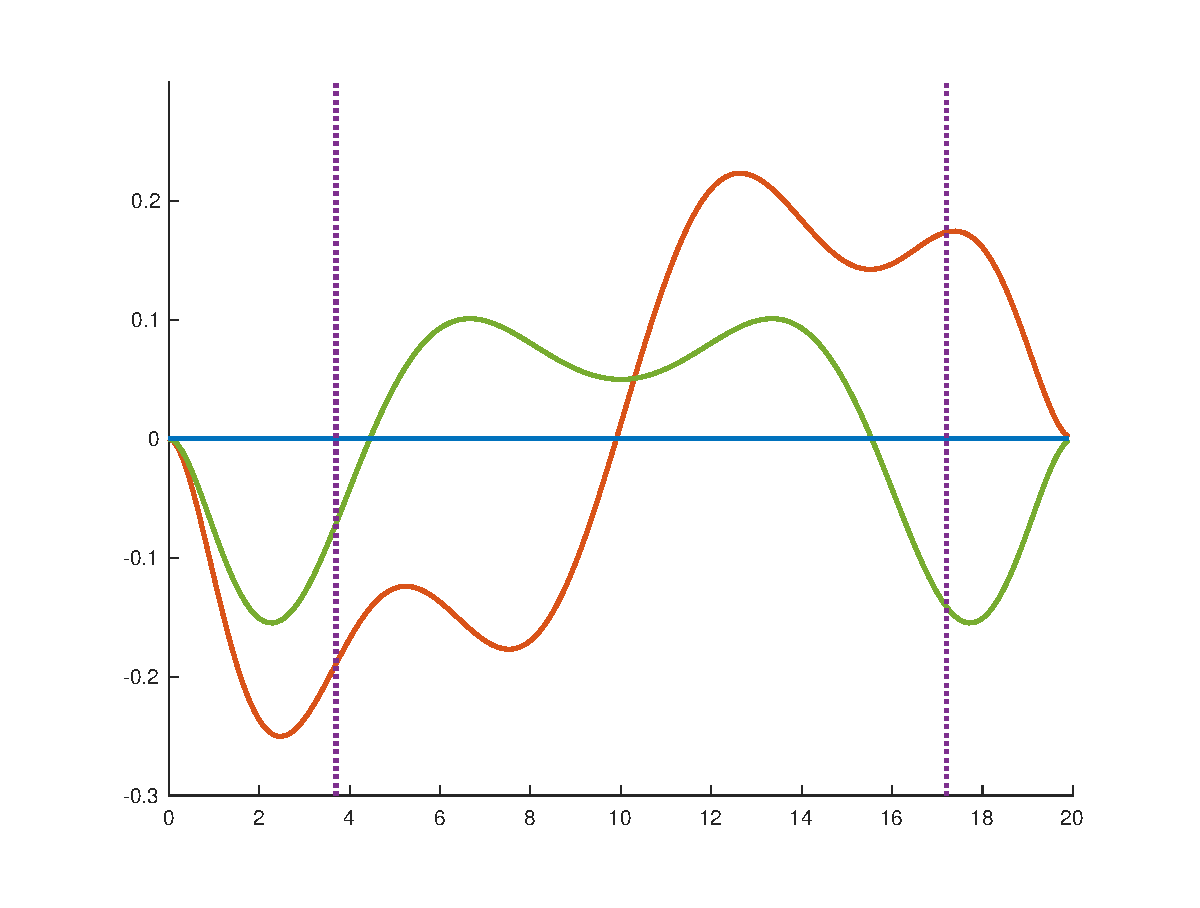
\includegraphics[width = 1.05\textwidth]{Figs/Chapter6/replan_init_acc.eps}}
		\end{minipage}
		\begin{minipage}{.45\linewidth}
			\centering
			\subfloat[]{%
				\label{FIG:REPLANNING-RESULTS-ACCELERATION-B}%
				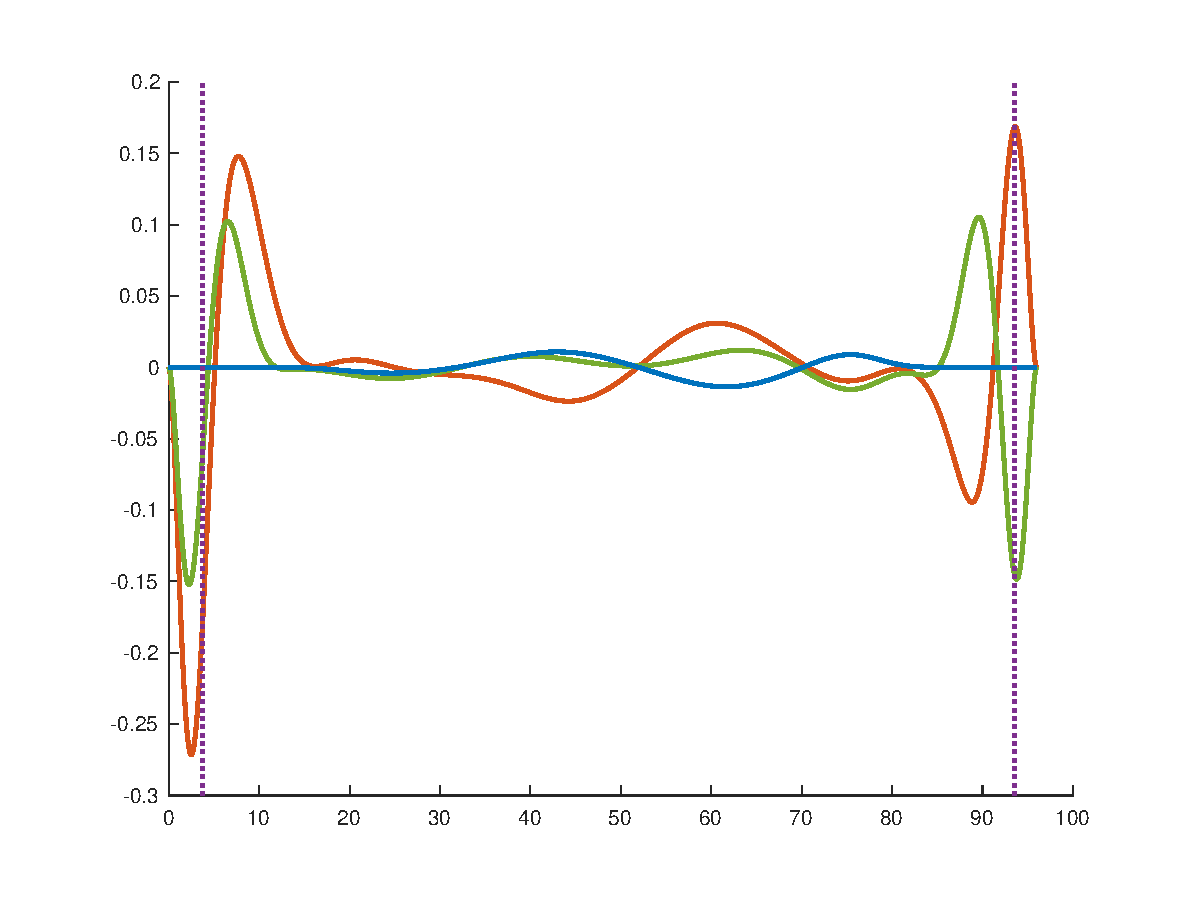
\includegraphics[width = 1.05\textwidth]{Figs/Chapter6/replan_post_acc.eps}}
		\end{minipage}
	\end{center}
	\caption{Initial acceleration trajectory (a) and replanned one (b).
    In the images, the red line represents the acceleration along the x-axis, the green one is the acceleration along the y-axis,
    and the blue represents the acceleration along the z-axis. The two vertical purple lines mark the initial and final cutting
    points, where the initial trajectory is broken and reconnected with the replanned one. Note that the acceleration continuity
    is completely preserved. In both cases the acceleration is kept below the safe level of $0.5m/s$.}%
    \label{FIG:REPLANNING-RESULTS-ACCELERATION}
\end{figure}
%%%%%%%%%%
%%%%%%%%%%
\begin{figure}[!t]
	\begin{center}
		\begin{minipage}{.45\linewidth}
			\centering
			\subfloat[]{%
				\label{FIG:REPLANNING-RESULTS-JERK-A}%
				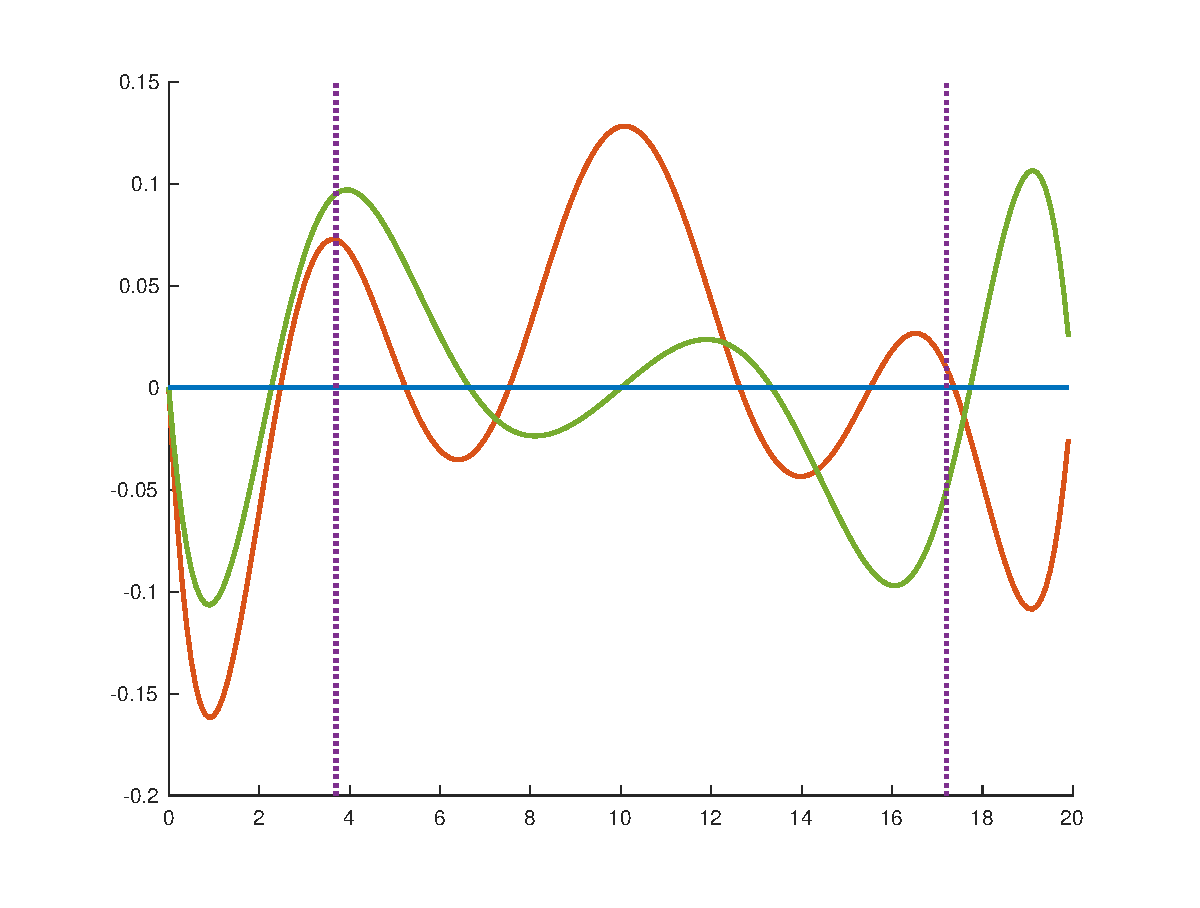
\includegraphics[width = 1.05\textwidth]{Figs/Chapter6/replan_init_jerk.eps}}
		\end{minipage}
		\begin{minipage}{.45\linewidth}
			\centering
			\subfloat[]{%
				\label{FIG:REPLANNING-RESULTS-JERK-B}%
				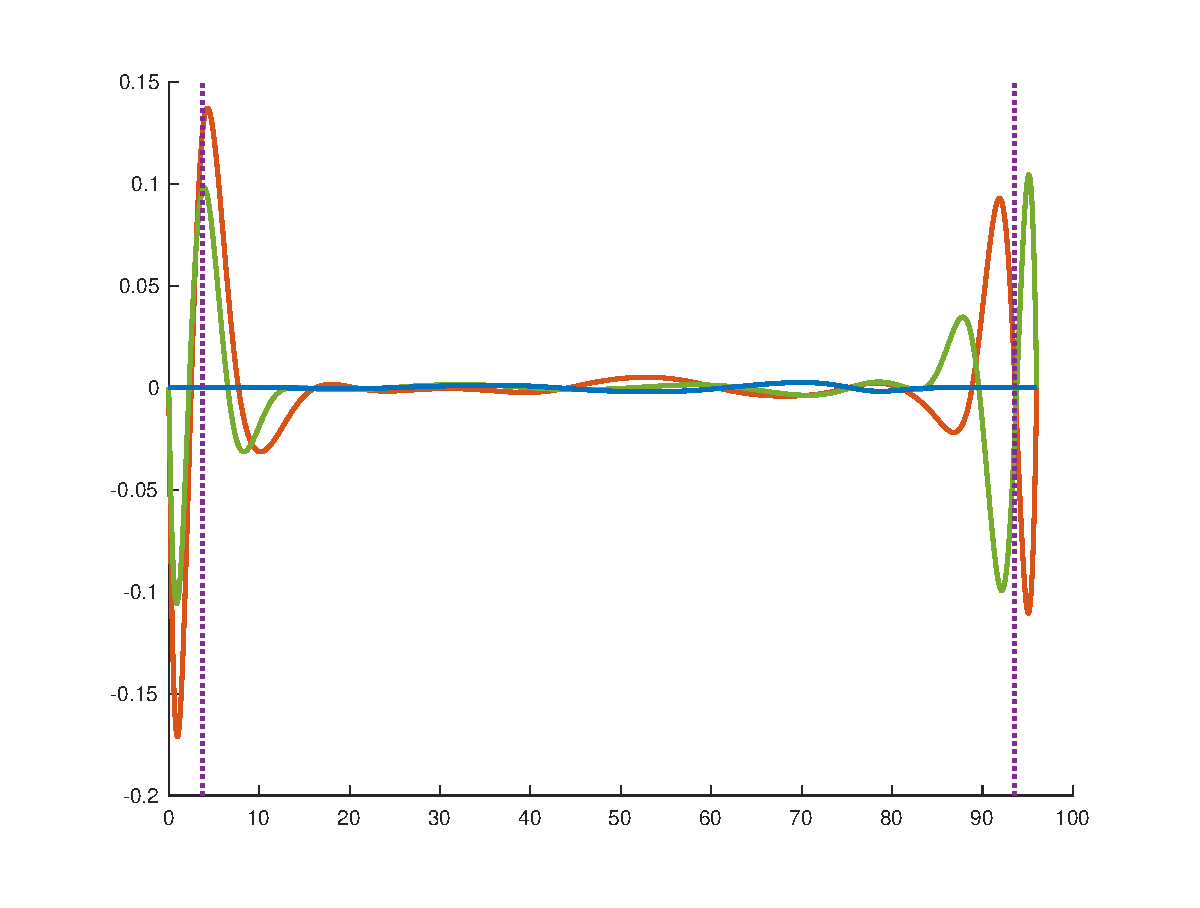
\includegraphics[width = 1.05\textwidth]{Figs/Chapter6/replan_post_jerk.eps}}
		\end{minipage}
	\end{center}
	\caption{Initial jerk trajectory (a) and replanned one (b).
    In the images, the red line represents the jerk along the x-axis, the green one is the jerk along the y-axis,
    and the blue represents the jerk along the z-axis. The two vertical purple lines mark the initial and final cutting
    points, where the initial trajectory is broken and reconnected with the replanned one. Note that the jerk continuity
    is completely preserved. No jerk limits have been fixed in this simulation.}%
    \label{FIG:REPLANNING-RESULTS-JERK}
\end{figure}
%%%%%%%%%%
%%%%%%%%%%
\begin{figure}[!t]
	\begin{center}
		\begin{minipage}{.45\linewidth}
			\centering
			\subfloat[]{%
				\label{FIG:REPLANNING-RESULTS-EXPLORATION-A}%
				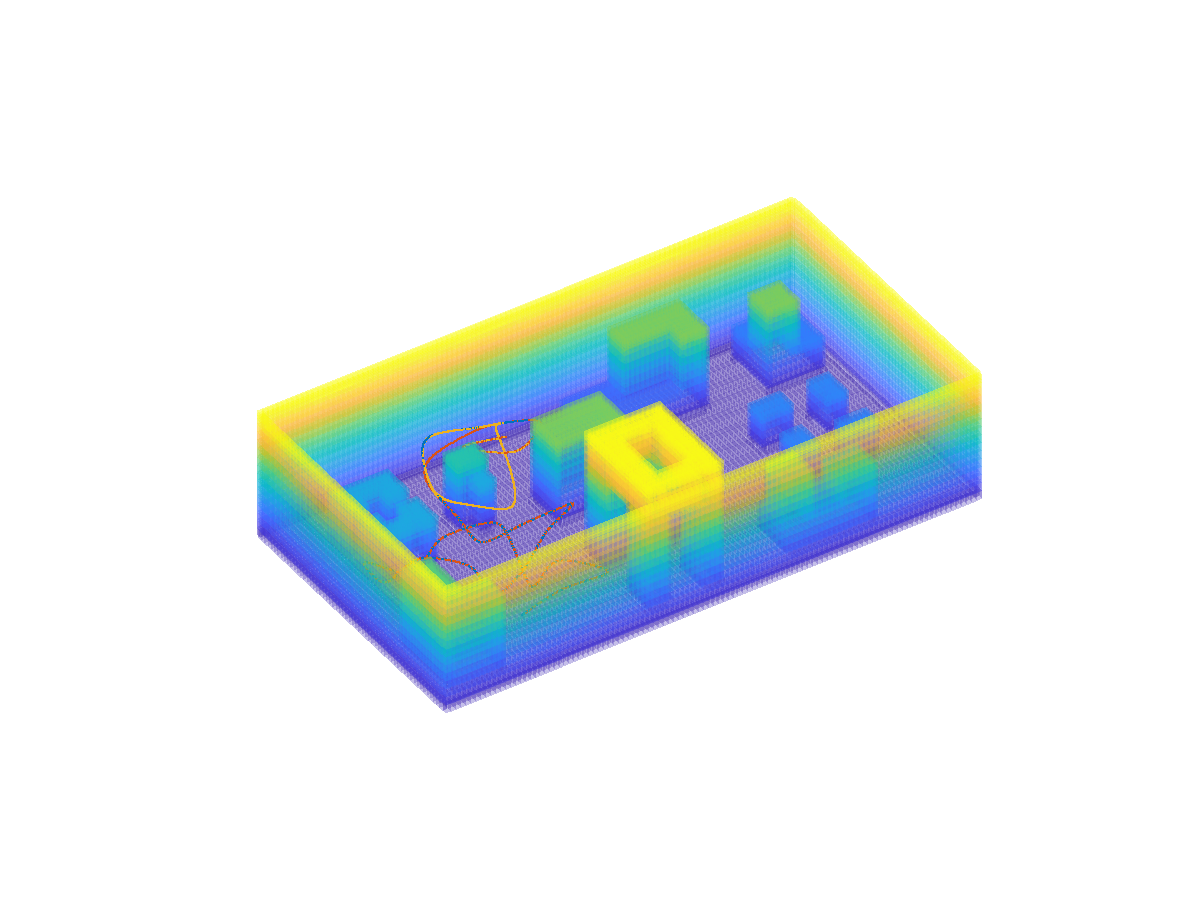
\includegraphics[trim={3.5cm 2.5cm 3cm 2.5cm}, clip = true, width = 1.05\textwidth]{Figs/Chapter6/replan_3d_traj_exploration_1.eps}}
		\end{minipage}
		\begin{minipage}{.45\linewidth}
			\centering
			\subfloat[]{%
				\label{FIG:REPLANNING-RESULTS-EXPLORATION-B}%
				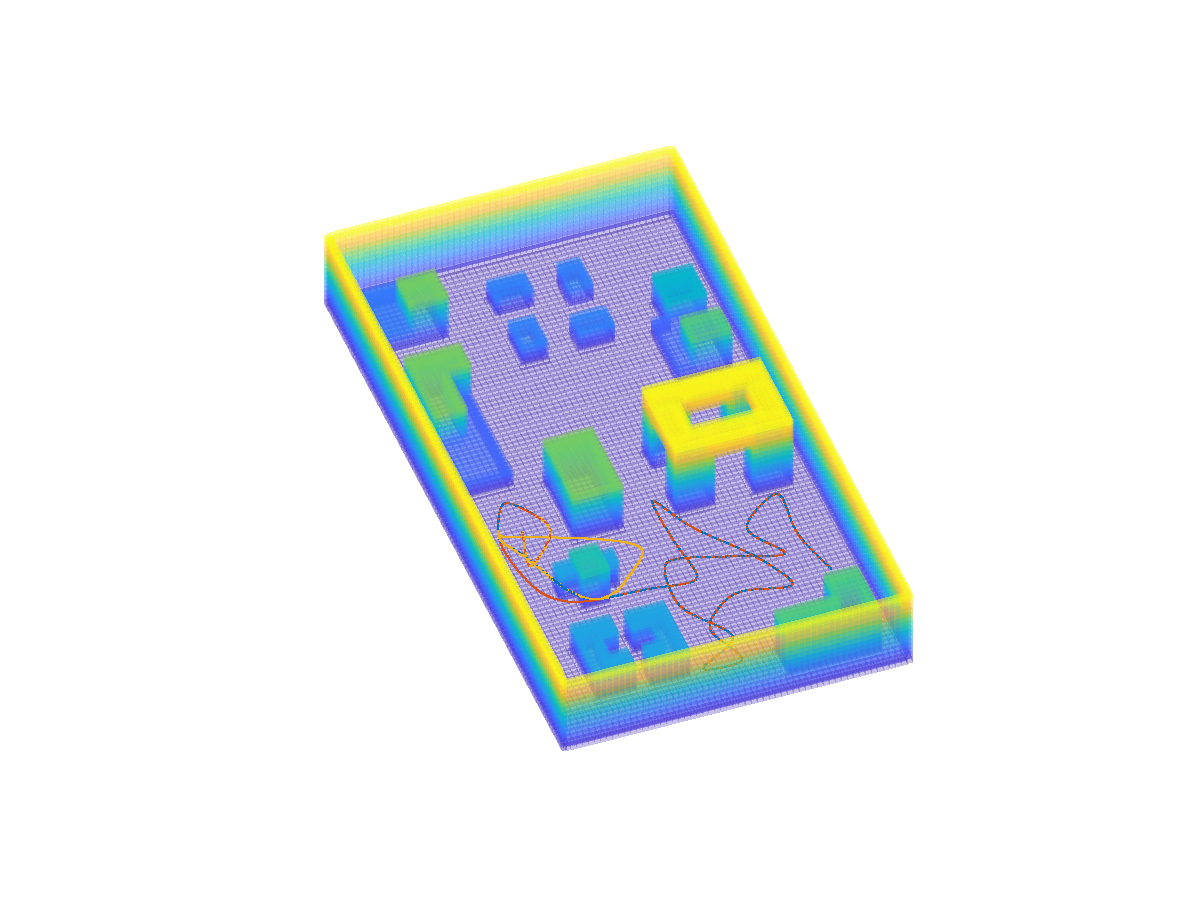
\includegraphics[trim={3.5cm 2.2cm 3cm 2.2cm}, clip = true, width = 1.05\textwidth]{Figs/Chapter6/replan_3d_traj_exploration.eps}}
		\end{minipage}
	\end{center}
	\caption{The reviewed approach applied to the specific case of exploration. In the image the trajectory has been replanned without a real
    collision in order to test its performance against previously unseen static obstacles, which may appear during the exploration task.
    As emerges from the figure, the replanning stack was able to successfully replan the exploring trajectory.}%
    \label{FIG:REPLANNING-RESULTS-EXPLORATION}
\end{figure}
%%%%%%%%%%
The proposed approach has been successfully applied to the synthetic environment proposed during the Leonardo drone challenge (see~\secref{SEC:DRONE-CONTEST}),
in two meaningful contexts. In the first stage, we supposed that the robot was performing a point-to-point trajectory to reach a particular area,
the committed initial trajectory was computed without the obstacles knowledge, leading to an unsafe motion. Next, we recreated the same 
exploration settings of~\secref{SEC:EXPLORATION-PROBLEM-DEFINITION}, where the robot was performing an exploration task driven by the
algorithm proposed in~\secref{SEC:SEARCH-PATROLLING-PERSPECTIVE}. In this second case, the initial trajectory was computed using the
environment knowledge, thus the performed trajectory was not in collision with obstacles, in order to trigger the replanning procedure
we inject a false sensor update containing an obstacle exactly on the motion direction.
The obtained results are reported in~\figref{FIG:REPLANNING-RESULTS-TRAJECTORY} for the first case, and in~\figref{FIG:REPLANNING-RESULTS-EXPLORATION}
for the exploration case. In both the images is reported the environment occupancy map, the initial trajectories, the optimised ones, and the sampled nodes.
In particular, the red continuous line represents the initial colliding motion, which requires replanning, in~\figref{FIG:REPLANNING-RESULTS-TRAJECTORY}
the collision is particularly clear, while in~\figref{FIG:REPLANNING-RESULTS-EXPLORATION} the red path is not colliding with any obstacles due to the
false measurement injected. The green circles represent the topologically different sampled and then shortened paths, the yellow lines are the 
trajectories obtained after path-guided optimisation, and the blue line is the final selected trajectory.
As the reader can notice, the blu line is always overlapped to the red one in the beginning end at the end, while is overlapped to the
yellow one inside the replanned segment. Figures~\ref{FIG:REPLANNING-RESULTS-VELOCITY},~\ref{FIG:REPLANNING-RESULTS-ACCELERATION},
and~\ref{FIG:REPLANNING-RESULTS-JERK} show the behavior of velocity, acceleration, and jerk before and after replanning.
In the images, the red lines are the quantities along the x-axis, the green ones are the same quantities along the y-axis, and the
z-axis is shown in blue. The purple vertical lines remark the start and goal points, where the initial colliding trajectory has been broken.
Note how the continuity is preserved, among the different trajectory segments, up to the chosen trajectory order $\order$.
A full list of parameters used to carry out the aforementioned simulations is reported in~\tabref{TAB:REPLANNING-PARAMETERS}.
%%%%%%%%%
{
\renewcommand{\arraystretch}{1.35}
\begin{table}[b!]
    \centering
    \begin{tabular}{||c|c||c|c||}
        \hline
        \hline
        $v_{\text{max}}$ & $1.5m/s$ & $a_{\text{max}}$ & $0.5m/s^2$ \\
        \hline
        $T_{\text{max}}$ & $2.0s$ & $\Delta_T$ & $0.1s^2$ \\
        \hline
        $T_{\text{min}}$ & $0.5s$ & $N_{\text{min}}$ & $3$ \\
        \hline
        $d_{\text{obs}}$ & $4m$ & $\Delta_{\text{max}}$ & $0.1s$ \\
        \hline
        $N_{\text{max}}$ & $3000$ & $d_{\text{res}}$ & $0.2m$ \\
        \hline
        $d_{\text{safe}}$ & $0.5m$ & $p$ & $7$ \\
        \hline
        $\lambda_1$ & $1.0$ & $\lambda_2$ & $10.0$ \\
        \hline
        \hline
    \end{tabular}
    \caption{Parameters used to test the replanning algorithm.}%
	\label{TAB:REPLANNING-PARAMETERS}
\end{table}}
%%%%%%%%%

%----------------------------------------------------------------------------------------
\section{Spatio-Temporal Curves Separation}%
\label{SEC:SPATION-TEMPORAL-SEPARATION} 
Despite the effectiveness of the replanning algorithm described in~\secref{SEC:REPLANNING-ALGORITHM}, it may fail in environments where
are present moving objects, as these are all treated as static obstacles. This simplifying assumption can be fatal to the replanning procedure
as the final trajectory may still be unsafe during the next time instant.
In this view, we proposed a novel approach to the replanning problem described in~\secref{SEC:REPLANNING-PROBLEM-DEFINITION}, in the
setting where the safe set is not fixed in time, thus moving obstacles may cross the robot motion.
The proposed solution is grounded on the assumption to have a priori knowledge of the surrounding environment, as well as an estimation
of the obstacle to which the agent may collides. We stress the fact that, even if we especially focus on the particular case of one single
moving obstacle, the proposed approach can easily extended to the multi-objects or multi-agent ones, where some of them are static.

Motivated by the success of GTO approaches~\cite{zhou2020robust, oleynikova2016continuous, gao2017gradient, usenko2017real}, and inspired by
the flexibility of B\acuteacc ezier curves in trajectory planning~\cite{gao2019flying, mehdi2015collision, park2020efficient}, we propose
a novel optimisation-based replanning paradigm where the B\acuteacc ezier parameterisation is employed twice in expressing the path and the associated timing law.
The final trajectory recalls the same structure chosen in~\secref{SEC:EXPLORATION-TRAJECTORY-PARAMETERISATION}, where the piecewise
structure allows for splitting the planning problem in several segments, and considering one environment area, or obstacle collision, at a time.
In the next sections we firstly remark how the double parameterisation is the key to fast plan optimal avoiding trajectories and state 
the final trajectory equations (\secref{SEC:ST-PARAM-COMPOSITION}), then we formulate the proposed solution as a single step optimisation
problem (\secref{SEC:ST-SEPARATION}).

\subsection{Spatio-Temporal Parameterisation \& Composition}%
\label{SEC:ST-PARAM-COMPOSITION}
%%%%%%%%%%
\begin{figure}[!t]
	\centering
	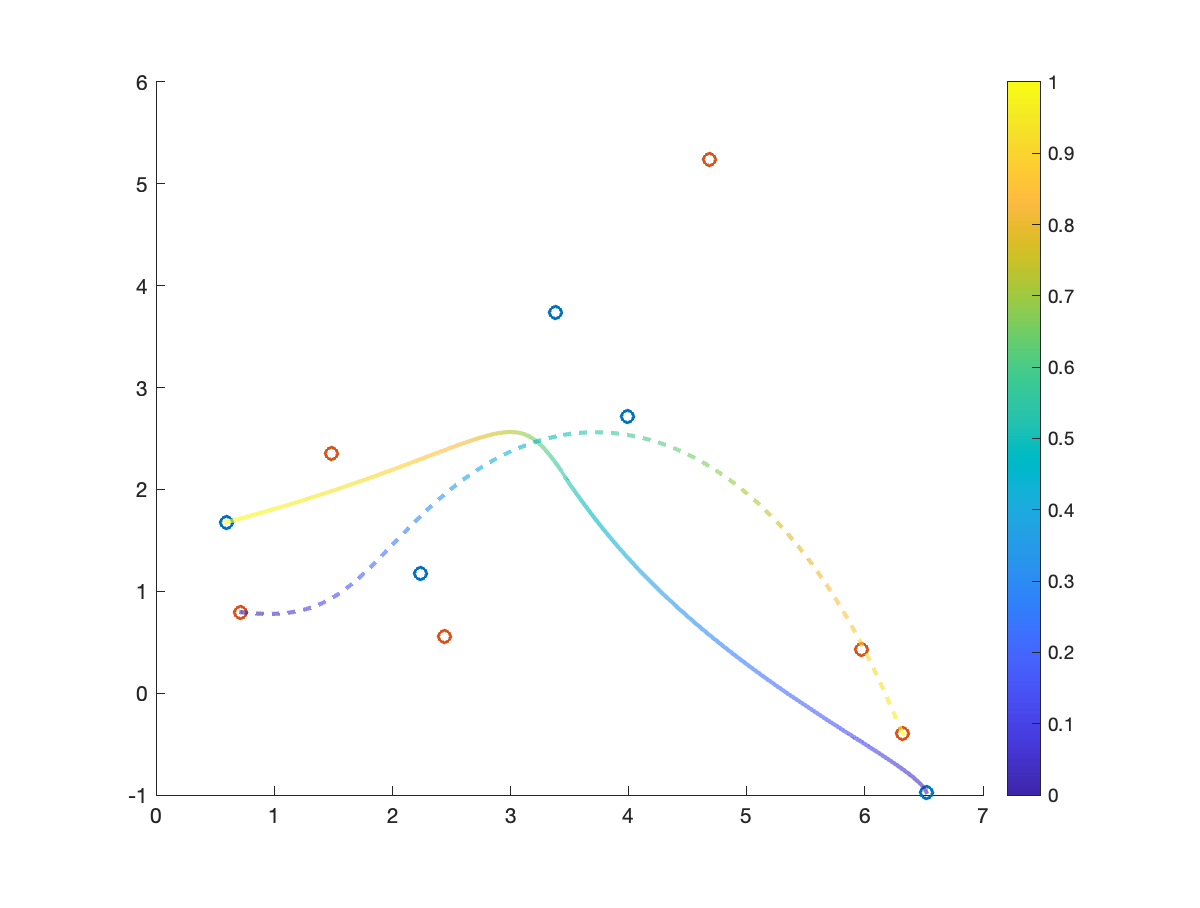
\includegraphics[width=0.6\textwidth]{Figs/Chapter6/st_bezier_timetraj_coll.eps}
	\caption{Example of two colliding B\acuteacc ezier curves. In the figure, the blue circles represent the randomly sampled
    control points of the continuous curve, while the red ones are the randomly sampled control points of the dotted one.
    The two curves are obtained as the composition of two B\acuteacc ezier curves of order $5$ for the position and $3$ for
    the timing law. The color shadows represent the time behavior of the two curves, normalized inside the interval $\lps 0, 1\rps$.}
	\label{FIG:ST-BEZIER-COLLIDING-TRAJ}
\end{figure}
%%%%%%%%%%
%%%%%%%%%%
\begin{figure}[!t]
	\centering
	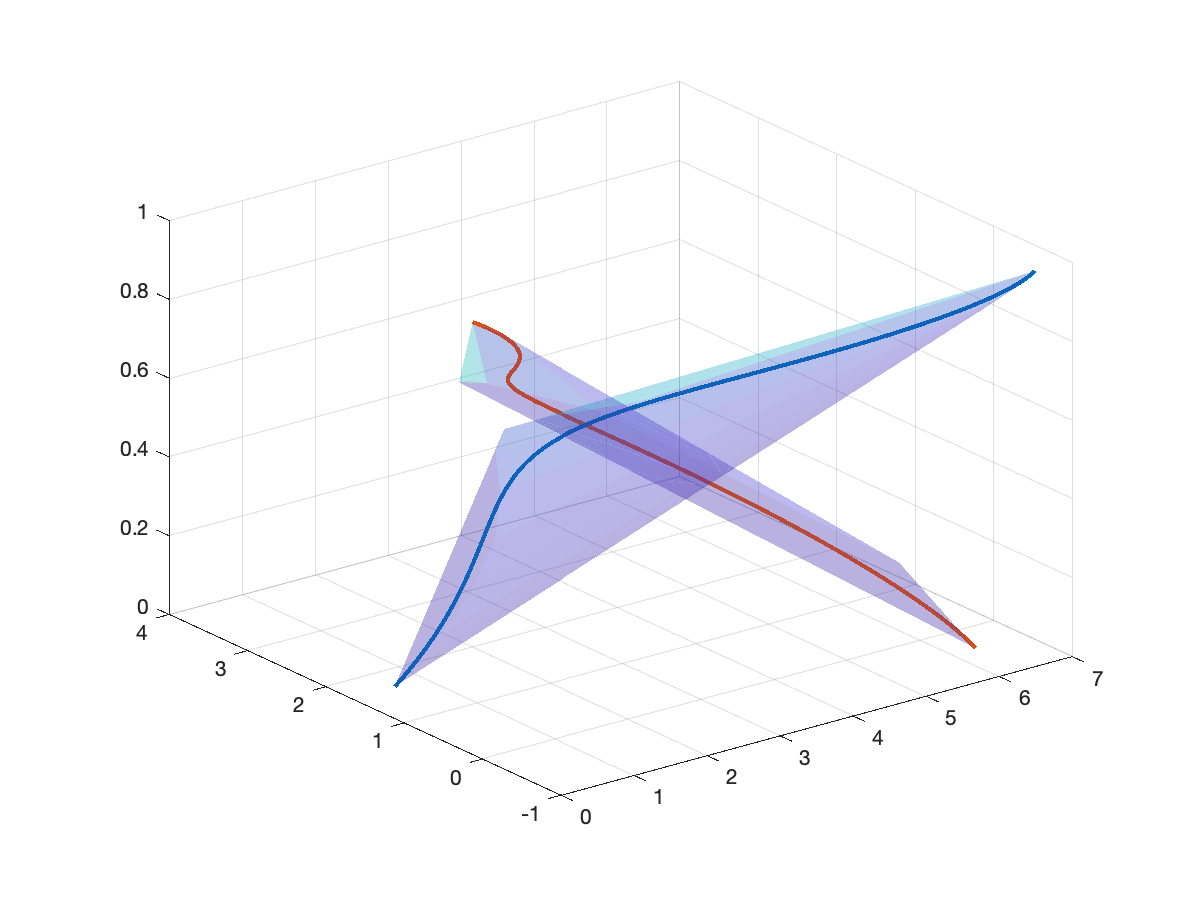
\includegraphics[width=0.6\textwidth]{Figs/Chapter6/st_bezier_convexhull_coll.eps}
	\caption{Convex hull representation of~\figref{FIG:ST-BEZIER-COLLIDING-TRAJ}. The third dimension is represented by the time,
    normalized inside the interval $\lps 0, 1\rps$.}
	\label{FIG:ST-BEZIER-COLLIDING-CONVEX}
\end{figure}
%%%%%%%%%%
The key idea behind the proposed solution is to parametrise both path and timing law by means of two B\acuteacc ezier curves.
In order to understand how this choice may helps during the planning stage, let us consider the example reported in~\figref{FIG:ST-BEZIER-COLLIDING-TRAJ}.
In this 2-dimensional case, two $5$-order B\acuteacc ezier curves
\begin{equation*}
    \begin{split}
        \rr & = \sum_{i = 0}^{\order} \bs{\cpoint}_i \basis_i^{\order} \lp \splinevar \rp, \\
        \rr^{o} & = \sum_{i = 0}^{\order} \bs{\cpoint}_i^{o} \basis_i^{\order} \lp \splinevar^{o} \rp,
    \end{split}
\end{equation*}
with $\order = 5$ and $\bs{\cpoint}_i$, $\bs{\cpoint}_i^{o}$ randomly sampled in $\R^2$.
The timing laws fixing $\splinevar$ and $\splinevar^{o}$ are chosen as other two B\acuteacc ezier curves ensuring the contidition
$\splinevar \in \lps 0, 1 \rps$ for any $t \in \R_{\ge 0}$
\begin{equation*}
    \begin{split}
        \splinevar & = \sum_{i = 0}^{\order_{\splinevar}} \splinevar_i \basis_i^{\order_{\splinevar}} \lp t \rp, \\
        \splinevar^{o} & = \sum_{i = 0}^{\order_{\splinevar}} \splinevar_i^{o} \basis_i^{\order_{\splinevar}} \lp t \rp.
    \end{split}
\end{equation*}
In the aforementioned relation, $\order_{\splinevar} = 3$, while $\splinevar_0 = \splinevar_0^o = 0$ and 
$\splinevar_{\order_{\splinevar}} = \splinevar_{\order_{\splinevar}}^o = 1$ to constraining $\splinevar, \splinevar^o \in \lps 0,1 \rps$.
The remaining free points have been selected randomly in $\R$.
In this settings, $\rr$ is thought of as the robot trajectory, while $\rr^{o}$ as the obstacle one.~\figref{FIG:ST-BEZIER-COLLIDING-TRAJ}
depicts the curves behavior on the $\R^2$ plane and along time thanks the reported colormap, in particular $\rr$ is depicted as a continuous line,
with the blue circles as associated control points, while $\rr^o$ is represented as a dotted line, with the orange circles as control points.
The reader can immediately recognize a possible collision around $0.5/0.6$ seconds, where the two lines cross each other.
The replanning problem may be solved just by moving the path control points $\bs{\cpoint}_i$, leading to a very huge detour from the initial
planned trajectory, or by slowing down the agent until its motion is safe from possible collisions.
In this second case, instead of moving the position control points we require to change the timing law, making the agent trajectory slower
and with a higher execution time. Although very appealing, the latter solution is not feasible as long as the relation between
the timing law and the induced agent-obstacle distance is not clear.
In this framework, the B\acuteacc ezier curve properties help us in formalizing such a relation exploiting first the composition rule,
then the difference rule, and finally the product one. Although the reader can find a complete analysis in~\secref{SEC:SPLINES-APPENDIX},
we recall here these properties applied to the considered specific case.
Let us suppose we want formalize the agent-obstacle squared distance $d \lp t \rp$ as a B\acuteacc ezier curve, whose control points $d_i$ must
be function of the initial quantities $\bs{\cpoint}_i$, $\bs{\cpoint}_i^o$, $\splinevar_i$, and $\splinevar_i^o$.
Applying the composition rule to $\rr$ and $\splinevar$, and $\rr^o$ and $\splinevar^o$ leads to
\begin{equation}%
    \label{EQ:ST-BEZIER-COMPOSITION-A}
    \begin{split}
        \bs{\cpoint}_{\splinevar_i} & = \lambda_{0,j}^{\order} \hspace{0.3cm} j = 0, \dots, \order \order_{\splinevar}, \\
        \bs{\cpoint}_{\splinevar_i}^o & = \rho_{0,j}^{\order} \hspace{0.3cm} j = 0, \dots, \order \order_{\splinevar},
    \end{split}
\end{equation}
where
\begin{equation}%
    \label{EQ:ST-BEZIER-COMPOSITION-B}
    \begin{split}
        \lambda_{i,j}^k =
        \begin{pmatrix}
            k \order_{\splinevar} \\ j
        \end{pmatrix}^{-1}
        \sum_{l = \max \lp 0, j - \order_{\splinevar} \rp}^{\min \lp j, k \order_{\splinevar} - \order_{\splinevar} \rp} &
        \begin{pmatrix}
            k \order_{\splinevar} - \cpnumber_u \\ l
        \end{pmatrix}
        \begin{pmatrix}
            \order_{\splinevar} \\ j-l
        \end{pmatrix} \\
        & \lps \lp 1-\splinevar_{j-l} \rp \lambda_{i,l}^{k-1} + \splinevar_{j-l}\lambda_{i+1,l}^{k-1} \rps,
    \end{split}
\end{equation}
\begin{equation}%
    \label{EQ:ST-BEZIER-COMPOSITION-C}
    \begin{split}
        \rho_{i,j}^k =
        \begin{pmatrix}
            k \order_{\splinevar} \\ j
        \end{pmatrix}^{-1}
        \sum_{l = \max \lp 0, j - \order_{\splinevar} \rp}^{\min \lp j, k \order_{\splinevar} - \order_{\splinevar} \rp} &
        \begin{pmatrix}
            k \order_{\splinevar} - \cpnumber_u \\ l
        \end{pmatrix}
        \begin{pmatrix}
            \order_{\splinevar} \\ j-l
        \end{pmatrix} \\
        & \lps \lp 1-\splinevar^o_{j-l} \rp \rho_{i,l}^{k-1} + \splinevar^o_{j-l}\rho_{i+1,l}^{k-1} \rps,
    \end{split}
\end{equation}
for $k = 1, \dots, \order$, $i = 0, \dots, \order-k$, and $j = 0, \dots, k\order_{\splinevar}$ and setting
$\lambda_{i,0}^{0} = \bs{\cpoint}_i$. The obtained control points $\bs{\cpoint}_{\splinevar_i}$ and
$\bs{\cpoint}_{\splinevar_i}^o$ represent two new curves of order $\order \order_{\splinevar}$, encoding both
path and timing law, then the agent-obstacle distance, along the two axis, can be evaluated as
\begin{equation}%
    \label{EQ:ST-BEZIER-COMPOSITION-D}
    \bs{\cpoint}_{\Delta_i} = \bs{\cpoint}_{\splinevar_i} - \bs{\cpoint}_{\splinevar_i}^o \hspace{0.3cm} \forall i = 0, \dots, \order \order_{\splinevar}.
\end{equation}
The final step consists in converting the axis-wise distance, to a squared Euclidean one.
To do this, $\bs{\cpoint}_{\Delta_i} = \lps \bs{\cpoint}_{\Delta_i}^x, \bs{\cpoint}_{\Delta_i}^y\rps$
must be first decomposed alog the two axis, then each component must be squared up as
\begin{equation}%
    \label{EQ:ST-BEZIER-COMPOSITION-E}
    \lp \bs{\cpoint}_{\Delta_i}^k \rp^2 =
    \sum_{j = \max \lp 0, i-\order \order_{\splinevar}2 \rp}^{\min \lp \order \order_{\splinevar}, i \rp}
    \frac{
        \begin{pmatrix}
            \order \order_{\splinevar} \\ j
        \end{pmatrix}
        \begin{pmatrix}
            \order \order_{\splinevar} \\ i-j
        \end{pmatrix}
    }{
        \begin{pmatrix}
            2\order \order_{\splinevar} \\ i
        \end{pmatrix}
    }
    \bs{\cpoint}_{\Delta_j}^k \bs{\cpoint}_{\Delta_{i-j}}^k,
\end{equation}
with $k = x,y$ and $i = 0, \dots, 2\order \order_{\splinevar}$.
Finally, the squared Euclidean distance can be evaluated as a B\acuteacc ezier curve $d \lp t \rp$ of order $2\order \order_{\splinevar}$
with control points
\begin{equation}%
    \label{EQ:ST-BEZIER-COMPOSITION-F}
    d_i = \lp \bs{\cpoint}_{\Delta_i}^x \rp^2 + \lp \bs{\cpoint}_{\Delta_i}^y \rp^2.
\end{equation}
\begin{remark}
    Equations~\eqref{EQ:ST-BEZIER-COMPOSITION-A}-\eqref{EQ:ST-BEZIER-COMPOSITION-F} look complicated, but at the end, the relation
    between $d_i$ and $\bs{\cpoint}_i$, $\splinevar_i$, $\bs{\cpoint}_i^o$, and $\splinevar^o_i$ results to be a simple algebraic relation.
    Let define the map $\Gamma : \R^{2(\order+\order_{\splinevar})} \mapsto \R^{2 \order \order_{\splinevar}}$ as the function mapping the
    initial path and time control points to the final squared Euclidean distance.
\end{remark}
\begin{remark}
    Equations~\eqref{EQ:ST-BEZIER-COMPOSITION-A}-\eqref{EQ:ST-BEZIER-COMPOSITION-F} have been developed for a planar case,
    but the extension to the three-dimension case is straightforward, considering $\bs{\cpoint}, \bs{\cpoint}^o \in \R^3$ and
    $k = x,y,z$.
\end{remark}
The key idea behind the proposed approach lies in the possibility to separate the agent curve and the obstacle one both in space, and
time, letting the algorithm to select the optimal trade-off between moving the position control points, or the timing law ones.
The adopted B\acuteacc ezier parameterisation is crucial in this view since it allows to continuously keep separated the two curves, and
straightforwardly join them when is required. A graphical representation of this property is depicted in~\figref{FIG:ST-BEZIER-COLLIDING-CONVEX},
where is reported a convex hull representation of the colliding curves shown in~\figref{FIG:ST-BEZIER-COLLIDING-TRAJ}.
In~\figref{FIG:ST-BEZIER-COLLIDING-CONVEX} the two-dimensional curves are depicted in $\R^3$, with the time being the third axis.
This three-dimensional representation has been obtained enlarging the set of composed control points from~\eqqref{EQ:ST-BEZIER-COMPOSITION-A},
with $\splinevar_i$ and $\splinevar_i^o$. The resulting trajectories are still B\acuteacc ezier curves, thus the convex hull 
containment property still holds, and the obtained polyhedra can be used to verify collisions both in time and space.

We conclude this section by recalling the piecewise B\acuteacc ezier structure defined in~\secref{SEC:EXPLORATION-TRAJECTORY-PARAMETERISATION},
used here to represent the final quadcopter trajectory.
\begin{equation}%
    \label{EQ:ST-SEPARATION-PIECEWISE}
	\rr \lp t \rp=
	\begin{cases}
		\sum_{i=0}^{\order} \basis_i^{\order}(\splinevar_1 \lp \clock_1 \rp) \bs{\cpoint}^1_i & \hspace{-0.2cm} t \in [T_0, T_1],\\
		\sum_{i=0}^{\order} \basis_i^{\order}(\splinevar_2 \lp \clock_1 \rp) \bs{\cpoint}^2_i & \hspace{-0.2cm} t \in [T_1, T_2],\\
		\hspace{0.2cm} \vdots & \vdots \\
		\sum_{i=0}^{\order} \basis_i^{\order}(\splinevar_{\segnumber} \lp \clock_{\segnumber} \rp) \bs{\cpoint}^{\segnumber}_i & \hspace{-0.2cm} t \in [T_{\segnumber-1}, T_{\segnumber}],\\
	\end{cases}
\end{equation}
with $\clock_i = \frac{t-T_{i-1}}{T_{i}-T_{i-1}}$ and $\splinevar_j \lp \clock_j \rp = \sum_{i=0}^{\order_{\splinevar}} \basis_i^{\order_{\splinevar}}(\clock_j) \splinevar^j_i$.
From now on we suppose $\order = 5$ and $\order_{\splinevar} = 3$.

\subsection{Spatio-Temporal Separation}%
\label{SEC:ST-SEPARATION}
%%%%%%%%%%
\begin{figure}[!t]
	\begin{center}
		\begin{minipage}{.45\linewidth}
			\centering
			\subfloat[]{%
				\label{FIG:ST-BEZIER-2D-SETTING-A}%
				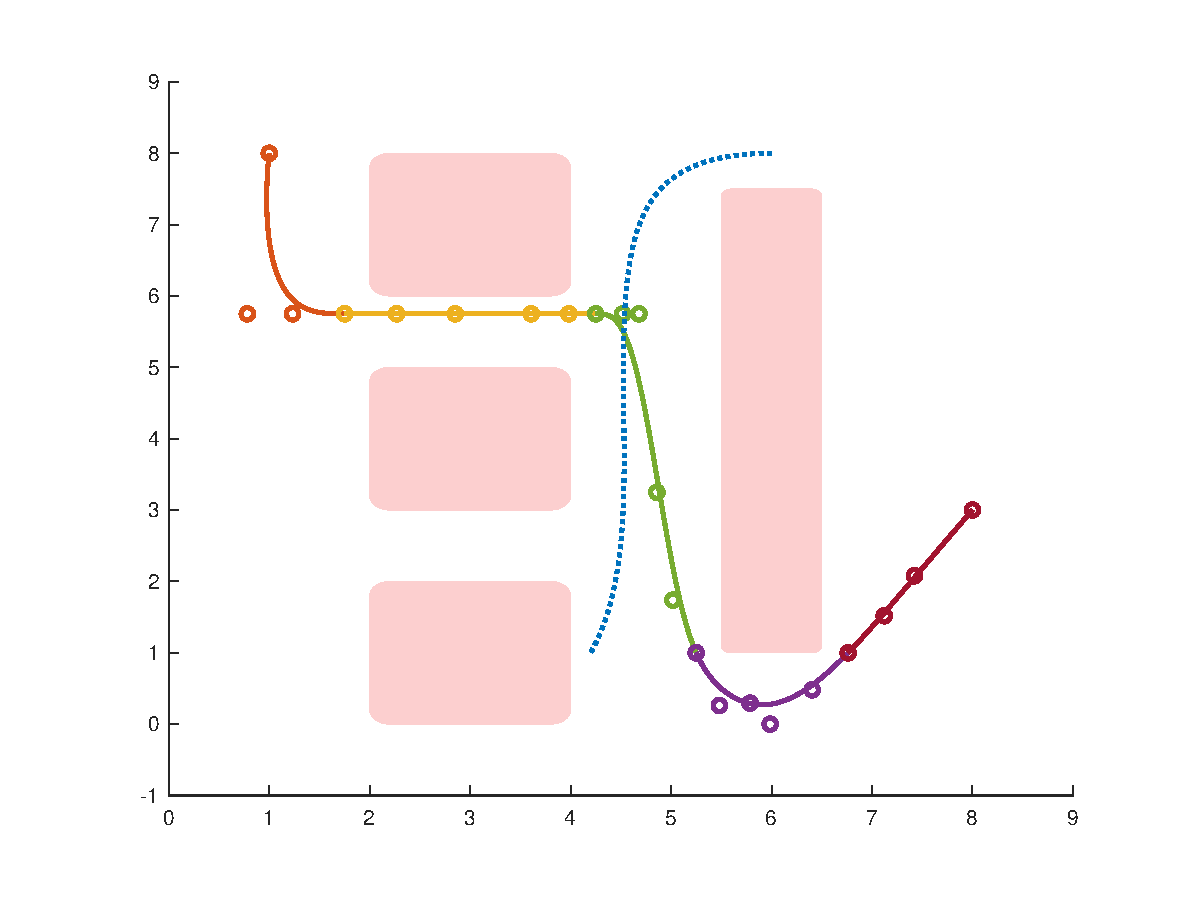
\includegraphics[width = 1.05\textwidth]{Figs/Chapter6/st_bezier_inital_setting_2d.eps}}
		\end{minipage}
		\begin{minipage}{.45\linewidth}
			\centering
			\subfloat[]{%
				\label{FIG:ST-BEZIER-2D-SETTING-B}%
				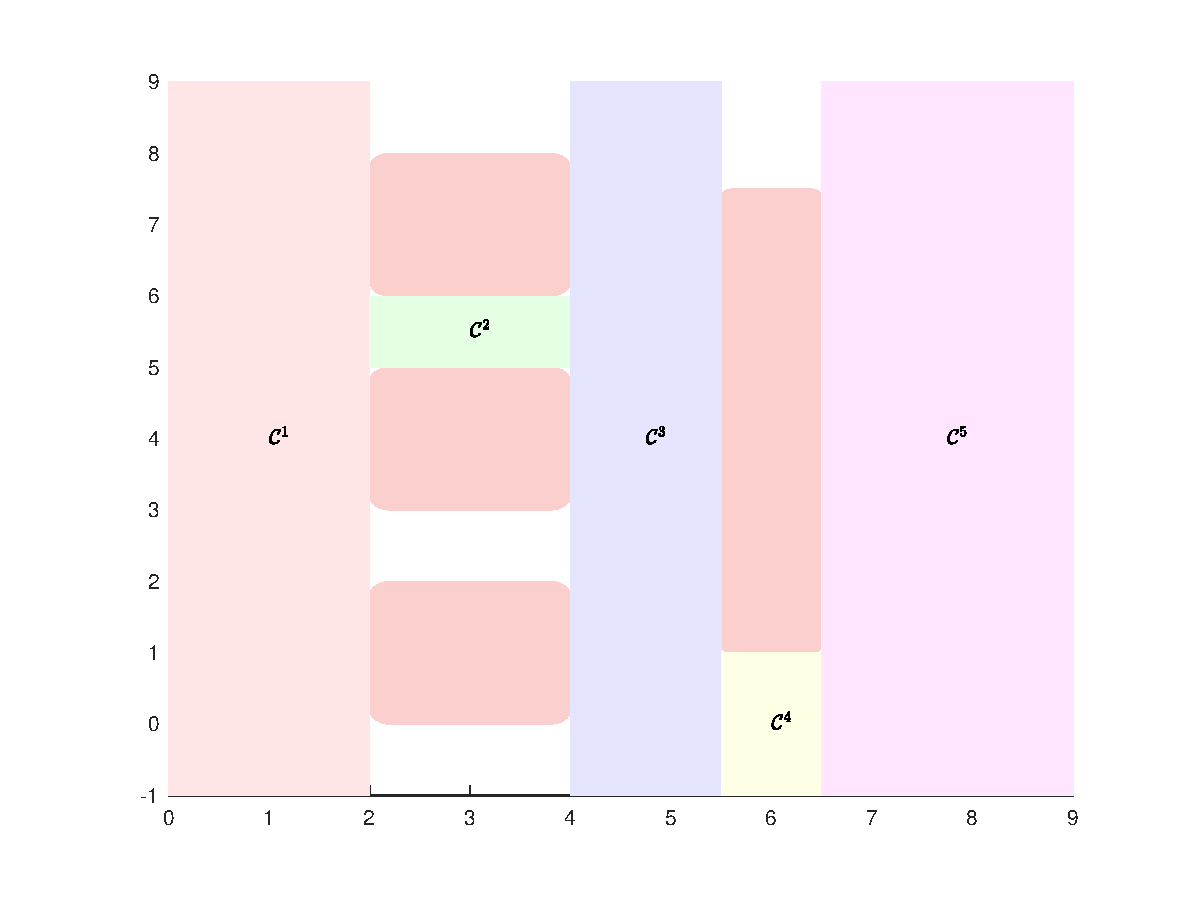
\includegraphics[width = 1.05\textwidth]{Figs/Chapter6/st_bezier_corridors_2d.eps}}
		\end{minipage}
	\end{center}
	\caption{Experimental setting used to test the proposed approach. Figure (a) depicts the initial trajectory planning made using the
    corridords depicted in image (b). The colored lines represent the initial agent trajectory, along with the respective selected control points,
    while the dotted blue line is the moving obstacle path, chosen in order to get in collision with the third green piece. The red 
    rectangles are environment obstacles assumed to be completely known.}%
    \label{FIG:ST-BEZIER-2D-SETTING}
\end{figure}
%%%%%%%%%%
%%%%%%%%%%
\begin{figure}[!t]
	\begin{center}
		\begin{minipage}{.45\linewidth}
			\centering
			\subfloat[]{%
				\label{FIG:ST-BEZIER-2D-INITIAL-A}%
				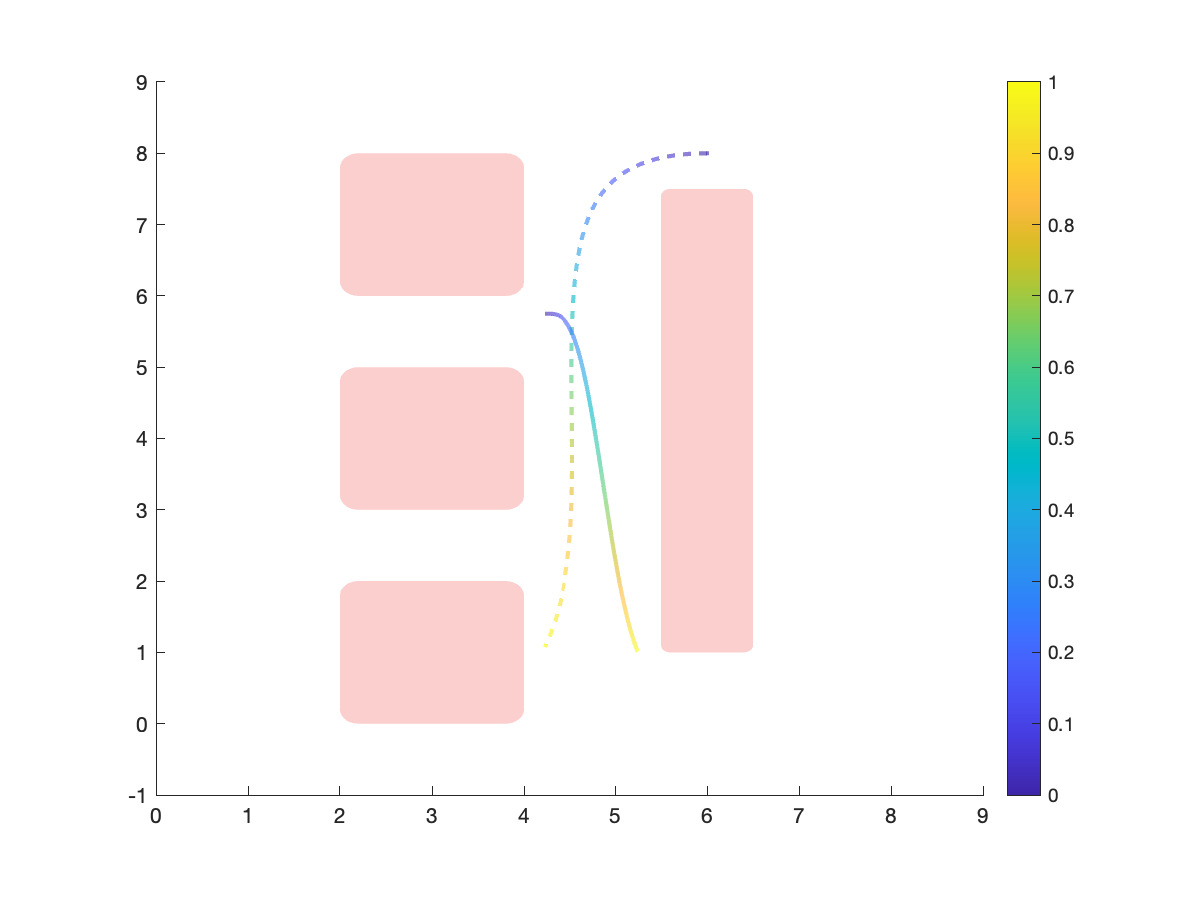
\includegraphics[width = 1.05\textwidth]{Figs/Chapter6/st_bezier_inital_2d.eps}}
		\end{minipage}
		\begin{minipage}{.45\linewidth}
			\centering
			\subfloat[]{%
				\label{FIG:ST-BEZIER-2D-INITIAL-B}%
				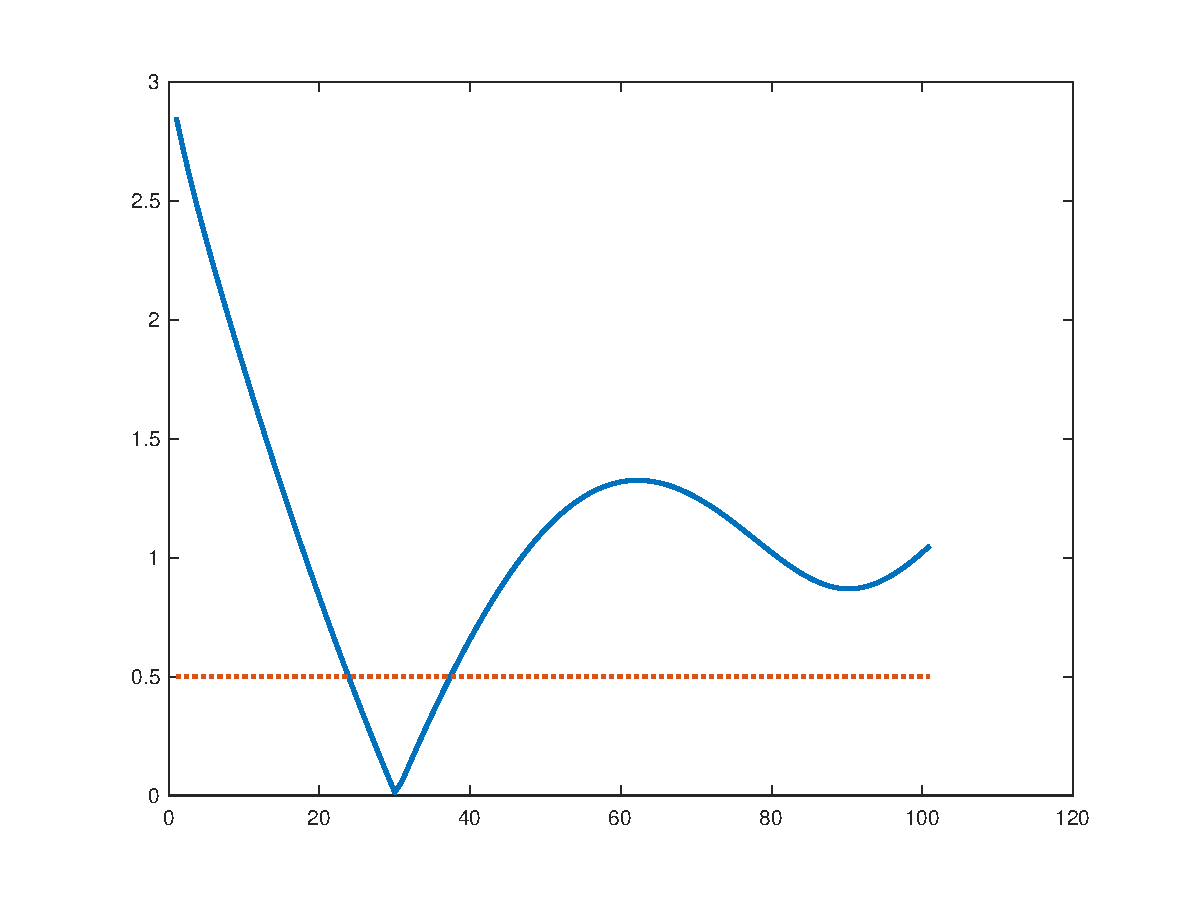
\includegraphics[width = 1.05\textwidth]{Figs/Chapter6/st_bezier_inital_distance_2d.eps}}
		\end{minipage}
	\end{center}
	\caption{Initial setting extrapolated from~\figref{FIG:ST-BEZIER-2D-SETTING}. In the left image, the two colliding pieces of
    trajectory are depicted with their behavior in time, normalized inside the interval $\lps 0,1 \rps$, while in the right image
    the blue line represents the agent-obstacle distance in time. The red dotted line, in the right image, is the chosen threshold
    for the minimum safe distance.}%
    \label{FIG:ST-BEZIER-2D-INITIAL}
\end{figure}
%%%%%%%%%%
With the previous analysis at hand, we propose here an optimisation-based approach to the replanning problem described
in~\secref{SEC:REPLANNING-PROBLEM-DEFINITION}, in the specific case where the obstacle trajectory $\rr_o \lp t \rp$ is known and
parameterised as a B\acuteacc ezier curve with control points $\cpoint_o^i$ for the path, and $\splinevar_o^i$ for the timing law.
In particular, let $\rr^j \lp t \rp$ the segment of~\eqqref{EQ:ST-SEPARATION-PIECEWISE} in (possible) collision with
the obstacle trajectory $\rr_o \lp t \rp$, then the problem of trajectory replanning can be solved as
\begin{equation}%
    \label{EQ:ST-SEPARATION-OPTIMISATION-PROBLEM}
    \begin{split}        
    \min_{
    \substack{\bs{\cpoint}_0, \dots, \bs{\cpoint}_{\order}; \\ \splinevar_0, \dots, \splinevar_{\order_{\splinevar}}}
    }
    & \loss
    \lp \bs{\cpoint}_0, \dots, \bs{\cpoint}_{\order}, \splinevar_0, \dots, \splinevar_{\order_{\splinevar}},
        \bs{\cpoint}^j_0, \dots, \bs{\cpoint}^j_{\order}, \splinevar^j_0, \dots, \splinevar^j_{\order_{\splinevar}} \rp \\
    \text{subj. to} \hspace{0.3cm} & \text{Continuity constraint}, \\
    & \text{Dynamical constraint}, \\
    & \text{Collision constraint},
    \end{split}
\end{equation}
with the constraints set depending on $\bs{\cpoint}^o_0, \dots, \bs{\cpoint}^o_{\order}, \splinevar^o_0, \dots, \splinevar^o_{\order_{\splinevar}}$.
The cost function $\loss \lp \cdot \rp$ can be chosen so as described in~\secref{SEC:REPLANNING-PROBLEM-DEFINITION}, recalling the
necessity to keep the replanned trajectory as close as possible to the original one
\begin{equation}%
    \label{EQ:ST-BEZIER-LOSS}
    \loss \lp \cdot \rp = \sum_{i=0}^{\order} \norm{\bs{\cpoint}_i - \bs{\cpoint}^j_i} + \sum_{i=0}^{\order_{\splinevar}} \lb \splinevar_i - \splinevar^j_i \rb,
\end{equation}
or so as described in~\secref{SEC:REPLANNING-OPTIMISATION}, including some trajectory regularisation terms.
In the following we briefly details and formulate the constraints in~\eqref{EQ:ST-SEPARATION-OPTIMISATION-PROBLEM}.
\begin{itemize}
    \item[\emph{Continuity}]\emph{constraint}.\\
    Belongs to this family of constraints all those conditions required to continuously connect the replanned trajectory segment with
    $\rr^{j-1}$ and $\rr^{j+1}$. In this context, we enforce continuity up to the third derivate, since higher order differentiations
    may complex the problem unnecessarily. Position continuity is easily obtained via control points matching as
    \begin{equation*}
        \begin{split}
            \splinevar_0 & = 0, \\
            \splinevar_{\order_{\splinevar}} & = 1, \\
            \rr_0 & = \rr_0^j, \\
            \rr_{\order} & = \rr_{\order}^j, \\
        \end{split}
    \end{equation*}
    where points denoted with apex $^j$ are the old control points.
    As regards velocity and acceleration continuity, we differentiate $\rr^j \lp t \rp$, with an eye to the composed stucture.
    \begin{equation*}
        \begin{split}
            \lp \rr_1 - \rr_0 \rp
            \lp \splinevar_1 - \splinevar_0 \rp & =
            \lp \rr^j_1 - \rr^j_0 \rp
            \lp \splinevar_1^j - \splinevar_0^j \rp, \\
            \lp \rr_{\order} - \rr_{\order-1} \rp
            \lp \splinevar_{\order_{\splinevar}} - \splinevar_{\order_{\splinevar}-1} \rp & =
            \lp \rr^j_{\order} - \rr^j_{\order-1} \rp
            \lp \splinevar_{\order_{\splinevar}}^j - \splinevar_{\order_{\splinevar}-1}^j \rp.
        \end{split}
    \end{equation*}
    \begin{equation*}
        \begin{matrix}
            \begin{matrix}
                \lp \rr_1 - \rr_0 \rp \lp \splinevar_2 - 2\splinevar_1 + \splinevar_0 \rp +
                \lp \rr_2 - 2\rr_1 + \rr_0 \rp \lp \splinevar_1 - \splinevar_0 \rp^2 = \\
                \lp \rr_1^j - \rr_0^j \rp \lp \splinevar_2^j - 2\splinevar_1^j + \splinevar_0^j \rp +
                \lp \rr_2^j - 2\rr_1^j + \rr_0^j \rp \lp \splinevar_1^j - \splinevar_0^j \rp^2,
            \end{matrix} \\
            \begin{matrix}
                \lp \rr_{\order} - \rr_{\order-1} \rp \lp \splinevar_{\order_{\splinevar}} - 2\splinevar_{\order_{\splinevar}-1} + \splinevar_{\order_{\splinevar}-2} \rp +
                \lp \rr_{\order} - 2\rr_{\order-1} + \rr_{\order-2} \rp \lp \splinevar_{\order_{\splinevar}} - \splinevar_{\order_{\splinevar}-1} \rp^2 = \\
                \lp \rr_{\order}^j - \rr_{\order-1}^j \rp \lp \splinevar_{\order_{\splinevar}}^j - 2\splinevar_{\order_{\splinevar}-1}^j + \splinevar_{\order_{\splinevar}-2}^j \rp +
                \lp \rr_{\order}^j - 2\rr_{\order-1}^j + \rr_{\order-2}^j \rp \lp \splinevar_{\order_{\splinevar}}^j - \splinevar_{\order_{\splinevar}-1}^j \rp^2.
            \end{matrix}
        \end{matrix}
    \end{equation*}

    \item[\emph{Dynamical}]\emph{constraint}.\\
    In the specific use case of quadcopter trajectory planning, differential flatness (\secref{SEC:DIFFERENTIAL-FLATNESS}) can be used to collapse
    the dynamics constraint to velocity and acceleration bounds.
    \begin{equation*}
        \begin{split}
            \order \order_{\splinevar} \lp \rr_{\splinevar_{i+1}} - \rr_{\splinevar_{i}} \rp / \lp T_{j+1} - T_j \rp & \le v_{\text{max}} \hspace{0.3cm} \forall i = 0, \dots, \order \order_{\splinevar}-1, \\
            \order \order_{\splinevar} \lp \order \order_{\splinevar} - 1 \rp \lp \rr_{\splinevar_{i+2}} - 2\rr_{\splinevar_{i+1}} + \rr_{\splinevar_{i}} \rp / \lp T_{j+1} - T_j \rp^2 & \le a_{\text{max}} \hspace{0.3cm} \forall i = 0, \dots, \order \order_{\splinevar}-2,
        \end{split}
    \end{equation*}
    with $\bs{\cpoint}_{\splinevar_{i}}$ be the $i$th control point of the composed curve~\eqref{EQ:ST-BEZIER-COMPOSITION-A}.
    Here we are exploiting the properties of closure with respect to composition and derivation, along with the convex hull containment one.
    In this context, as well as in the next collision constraint, the B\acuteacc ezier parameterisation plays a crucial role in
    simplifying the constraint formulation and dimensionality, leading to a manageable problem.

    \item[\emph{Collision}]\emph{constraint}.\\
    Finally, collision constraints are formulated as $n_{\text{c}}$ flght safe corridors for static obstacles avoidance,
    and as spatio-temporal distance for dynamic obstacle avoidance
    \begin{equation*}
        \begin{split}
            d_i & \ge d_{\text{safe}} \hspace{0.3cm} \forall i = 0, \dots, 2 \order \order_{\splinevar}, \\
            A^k \rr_i & \le b^k \hspace{0.3cm} \forall i = 0, \dots, \order, \hspace{0.3cm} \forall k = 0, \dots, n_{\text{c}}.
        \end{split}
    \end{equation*}
    In the aforementioned relation $d_i$ are the $2 \order \order_{\splinevar}$ control points defining the squared agent-obstacle
    distance, defined in~\eqqref{EQ:ST-BEZIER-COMPOSITION-F}, while $A^k$ and $b^k$ are $n_{\text{c}}$ convex polyhedra
    defining the safe regions free of static obstacles. In this setting, 
    \begin{equation*}
        \xset' = \bigcup_{k = 0}^{n_{\text{c}}} \left \{ \xx \in \R^{\dd{\xx}} : A^k \xx \le b^k \right \}.
    \end{equation*}
\end{itemize}
\begin{remark}
    The optimisation problem~\eqref{EQ:ST-SEPARATION-OPTIMISATION-PROBLEM} has been formulated for one agent only,
    colliding with a moving obstacle, the extension to the multi-agents case can be straightforwardly obtained by adding a new set
    of optimisation variables, describing the new agent trajectory.
\end{remark}

\subsection{Experimental Results}
%%%%%%%%%%
\begin{figure}[!t]
	\begin{center}
		\begin{minipage}{.45\linewidth}
			\centering
			\subfloat[]{%
				\label{FIG:ST-BEZIER-2D-U-RESULT-A}%
				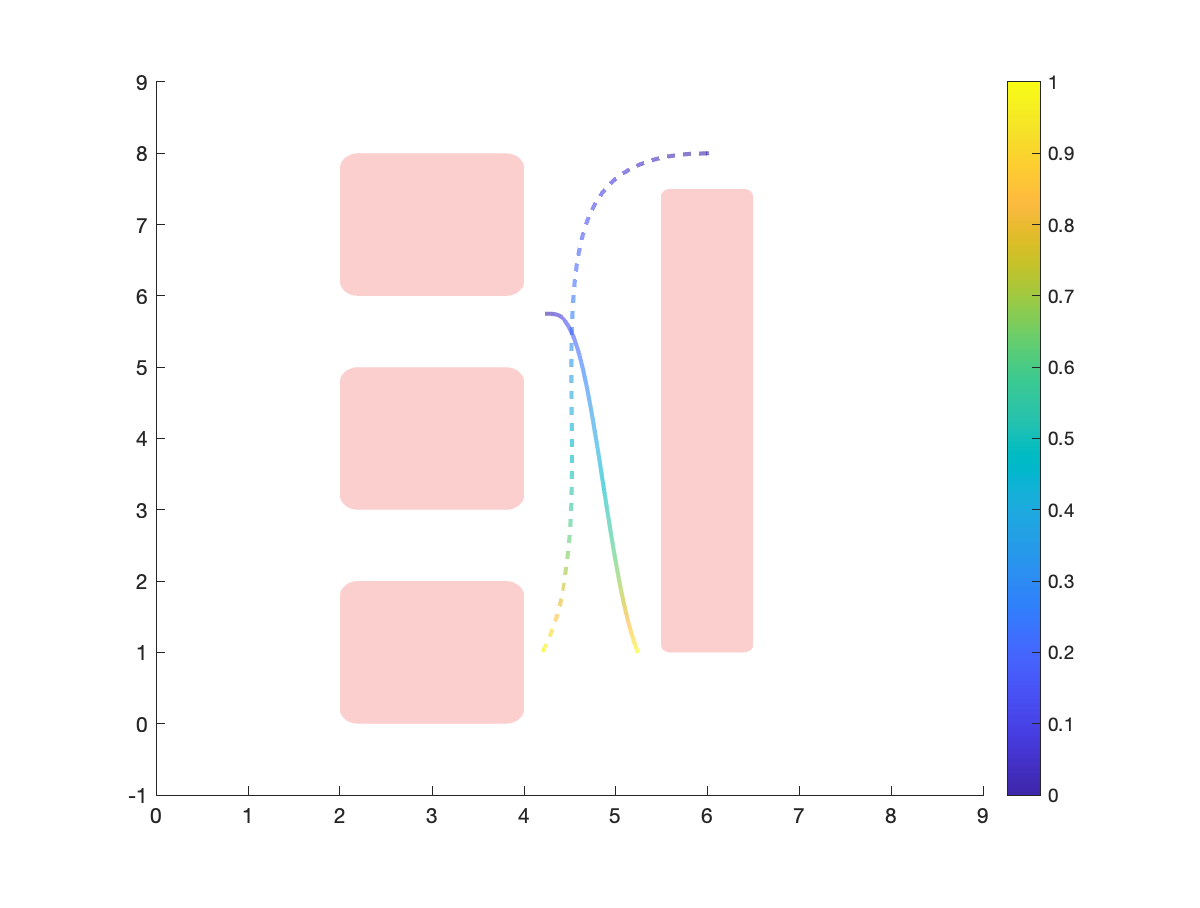
\includegraphics[width = 1.05\textwidth]{Figs/Chapter6/st_bezier_u_opt_2d.eps}}
		\end{minipage}
		\begin{minipage}{.45\linewidth}
			\centering
			\subfloat[]{%
				\label{FIG:ST-BEZIER-2D-U-RESULT-B}%
				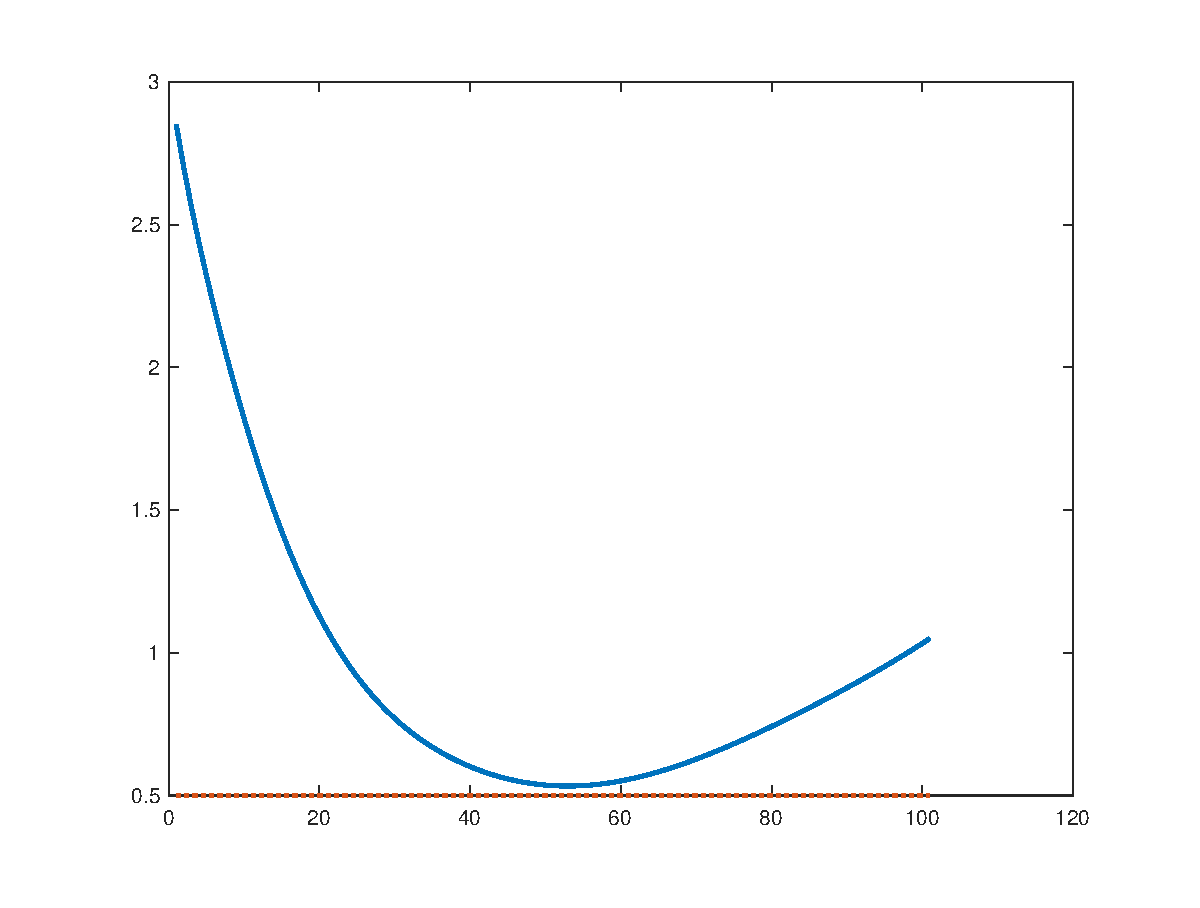
\includegraphics[width = 1.05\textwidth]{Figs/Chapter6/st_bezier_u_opt_distance_2d.eps}}
		\end{minipage}
	\end{center}
	\caption{Results of the proposed solution when used to optimise $\splinevar_i$ only.
    In the left image is depicted the same path as~\figref{FIG:ST-BEZIER-2D-INITIAL}, but with the new time behavior,
    normalized inside the interval $\lps 0,1 \rps$. The blue continuous line, in the right image, represents
    the new agent-obstacle distance, and the red dotted line is the fixed minimum safe distance.}%
    \label{FIG:ST-BEZIER-2D-U-RESULT}
\end{figure}
%%%%%%%%%%
%%%%%%%%%%
\begin{figure}[!t]
	\begin{center}
		\begin{minipage}{.45\linewidth}
			\centering
			\subfloat[]{%
				\label{FIG:ST-BEZIER-2D-PU-RESULT-A}%
				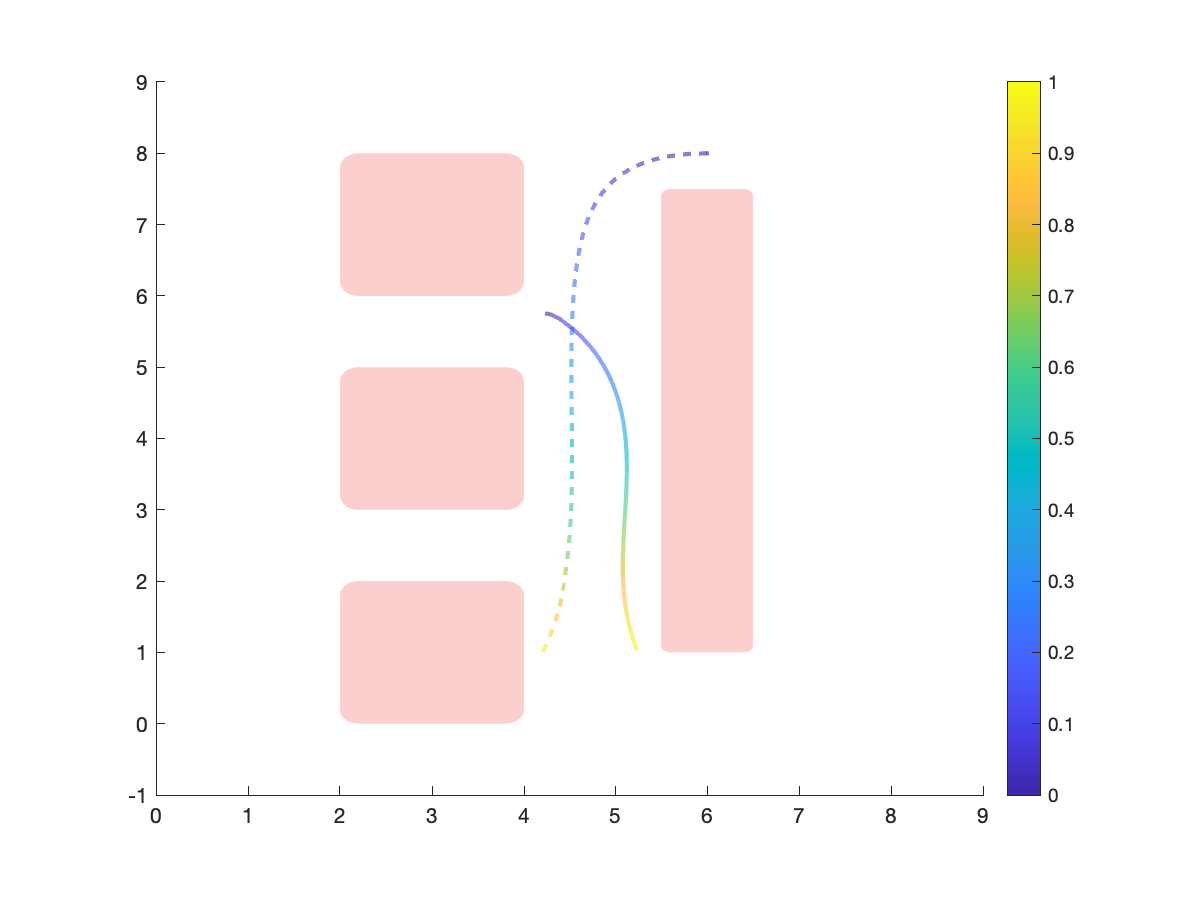
\includegraphics[width = 1.05\textwidth]{Figs/Chapter6/st_bezier_pu_opt_2d.eps}}
		\end{minipage}
		\begin{minipage}{.45\linewidth}
			\centering
			\subfloat[]{%
				\label{FIG:ST-BEZIER-2D-PU-RESULT-B}%
				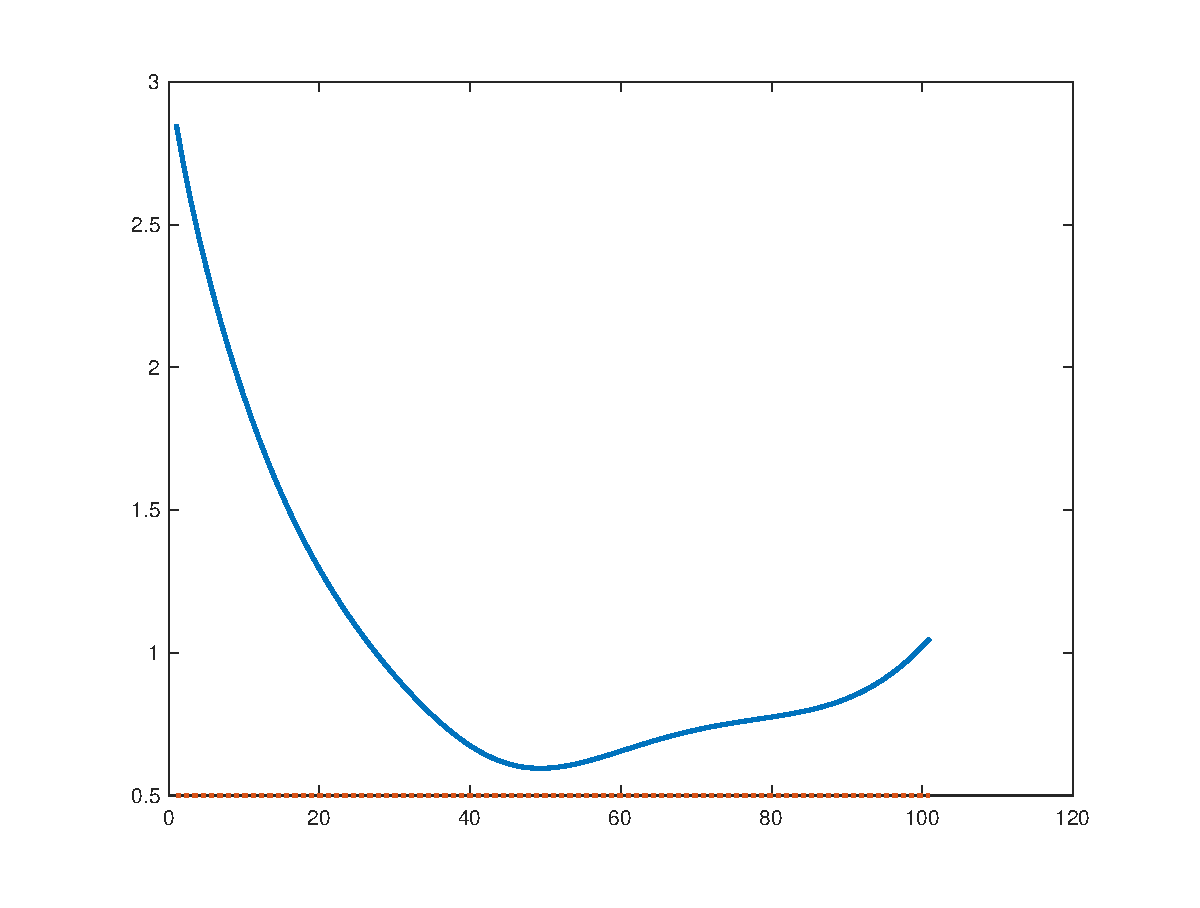
\includegraphics[width = 1.05\textwidth]{Figs/Chapter6/st_bezier_pu_opt_distance_2d.eps}}
		\end{minipage}
	\end{center}
	\caption{Results of the proposed solution when used to optimise both $\bs{\cpoint}_i$ and $\splinevar_i$.
    In the left image is depicted the new path with the new time behavior, normalized inside the interval $\lps 0,1 \rps$.
    The blue continuous line, in the right image, represents the new agent-obstacle distance, and the red dotted line is the
    fixed minimum safe distance.}%
    \label{FIG:ST-BEZIER-2D-PU-RESULT}
\end{figure}
%%%%%%%%%%
%%%%%%%%%%
\begin{figure}[!t]
	\begin{center}
		\begin{minipage}{.45\linewidth}
			\centering
			\subfloat[]{%
				\label{FIG:ST-BEZIER-3D-INITIALY-A}%
				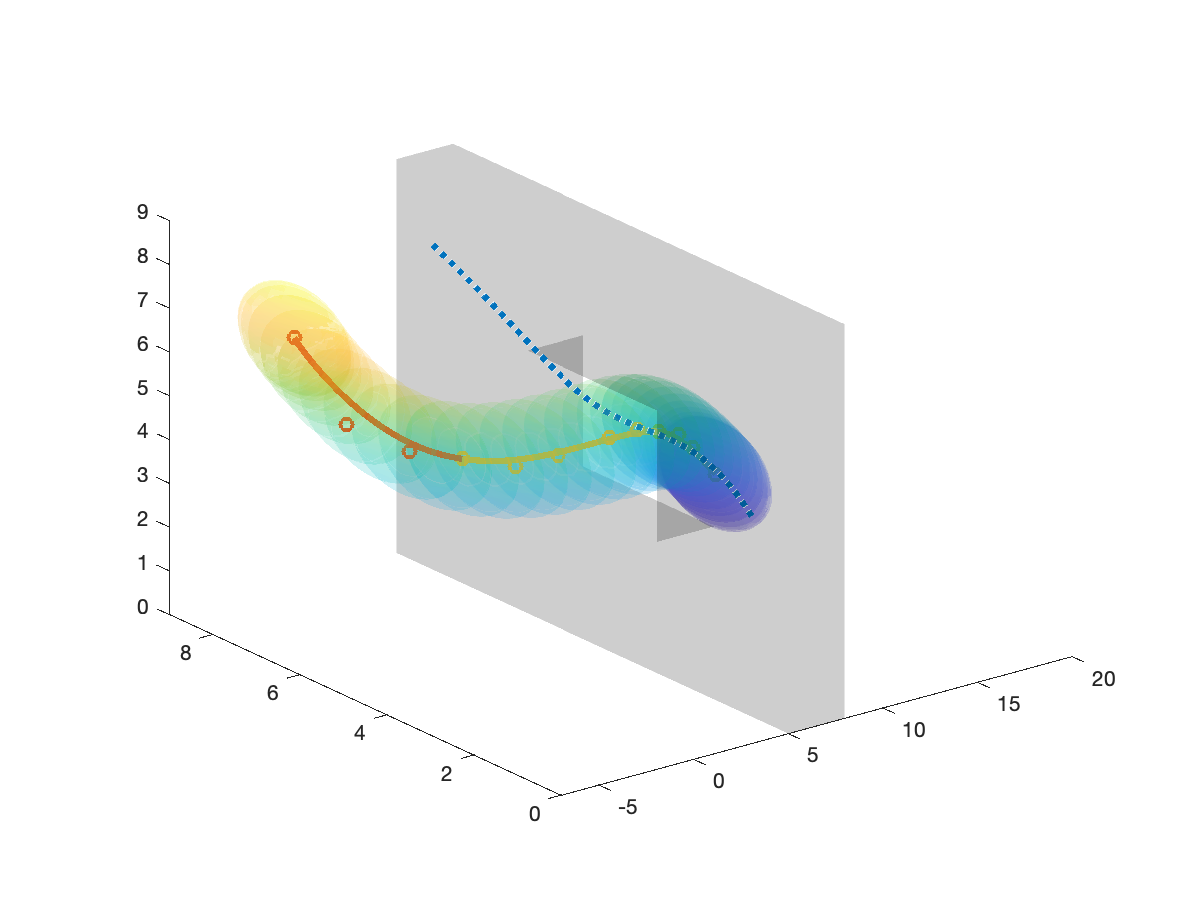
\includegraphics[width = 1.05\textwidth]{Figs/Chapter6/st_bezier_inital_setting_3d.eps}}
		\end{minipage}
		\begin{minipage}{.45\linewidth}
			\centering
			\subfloat[]{%
				\label{FIG:ST-BEZIER-3D-INITIAL-B}%
				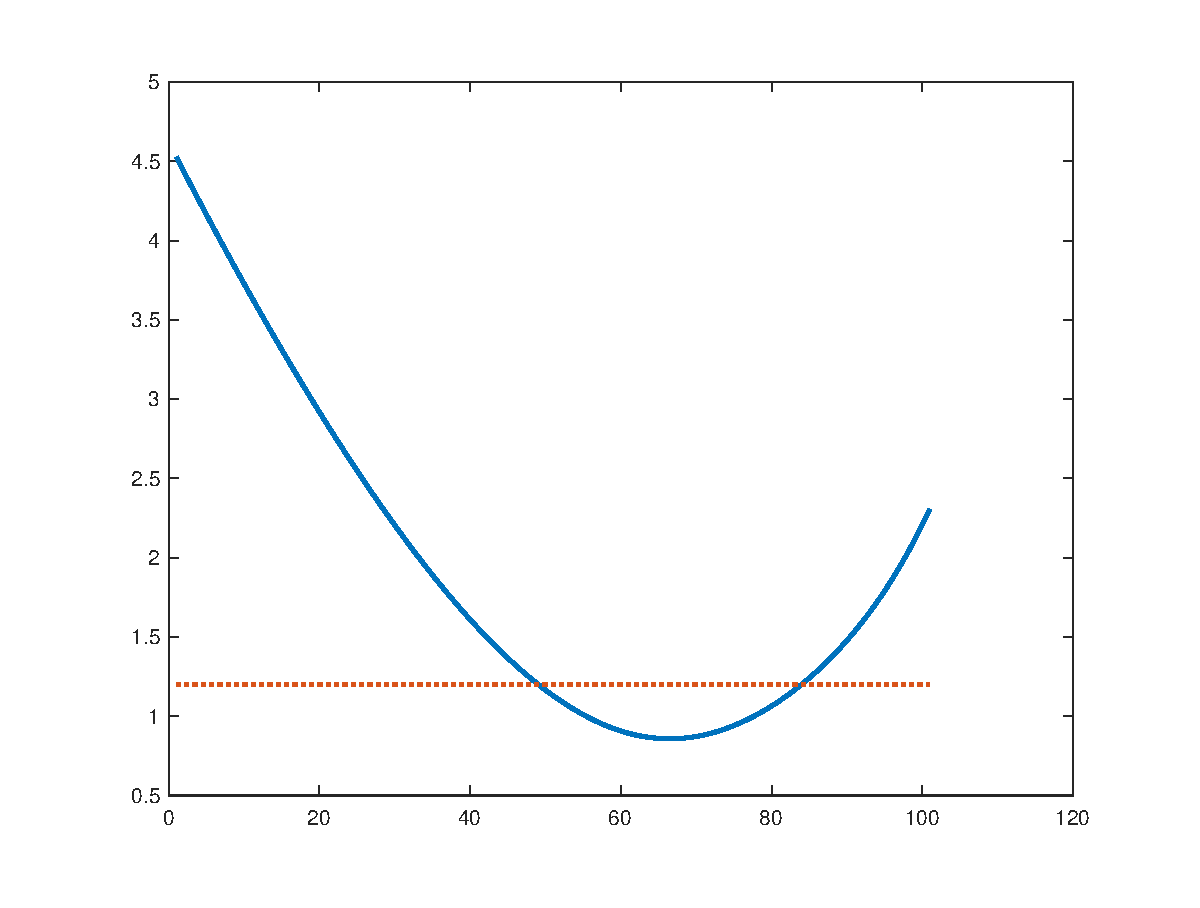
\includegraphics[width = 1.05\textwidth]{Figs/Chapter6/st_bezier_inital_distance_3d.eps}}
		\end{minipage}
	\end{center}
	\caption{Initial three-dimensional testing scenario. In the left image, the two colliding pieces of
    trajectory are depicted with the considered collision sphere. In the right image, the blue line represents the
    agent-obstacle distance in time, and the red dotted line is the chosen threshold for the minimum safe distance.}%
    \label{FIG:ST-BEZIER-3D-INITIAL}
\end{figure}
%%%%%%%%%%
%%%%%%%%%%
\begin{figure}[!t]
	\begin{center}
		\begin{minipage}{.45\linewidth}
			\centering
			\subfloat[]{%
				\label{FIG:ST-BEZIER-3D-U-RESULT-A}%
				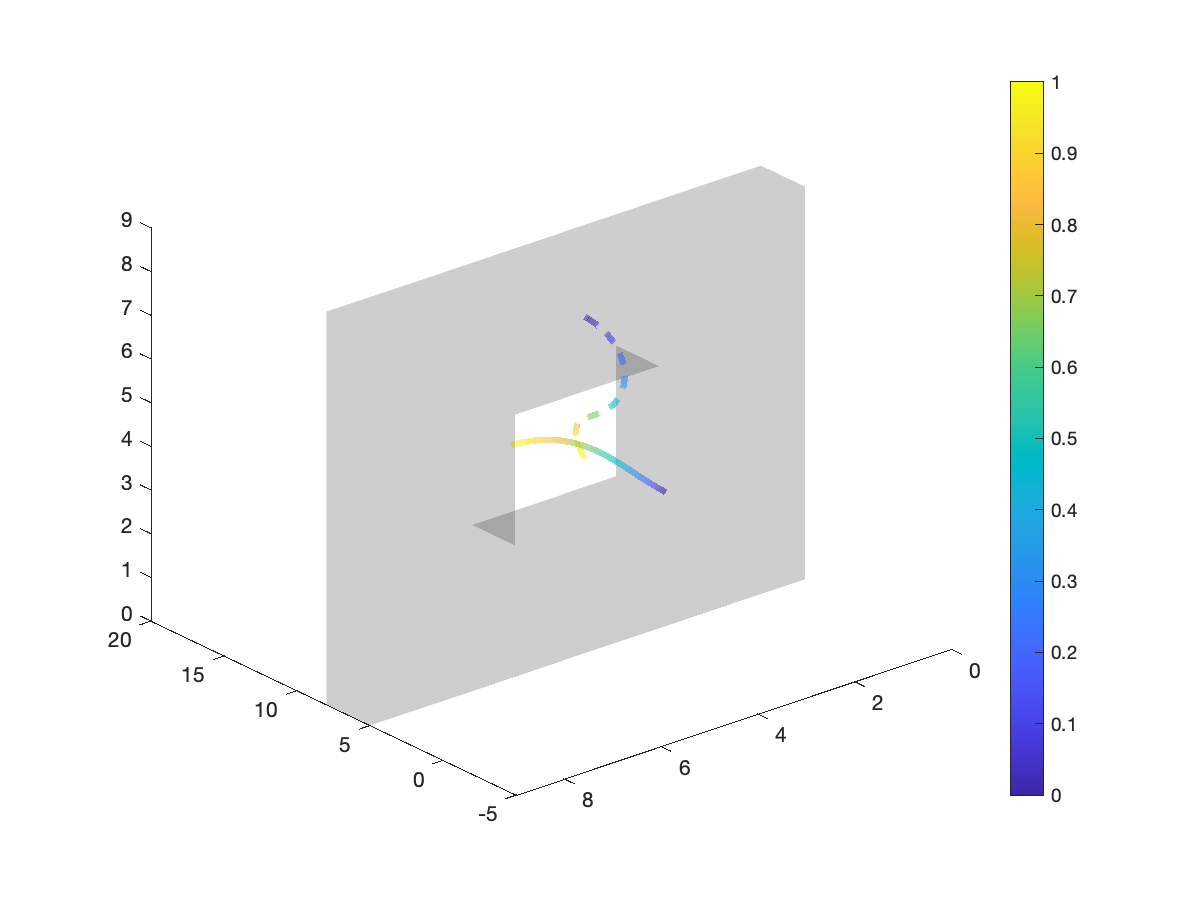
\includegraphics[width = 1.05\textwidth]{Figs/Chapter6/st_bezier_u_opt_3d.eps}}
		\end{minipage}
		\begin{minipage}{.45\linewidth}
			\centering
			\subfloat[]{%
				\label{FIG:ST-BEZIER-3D-U-RESULT-B}%
				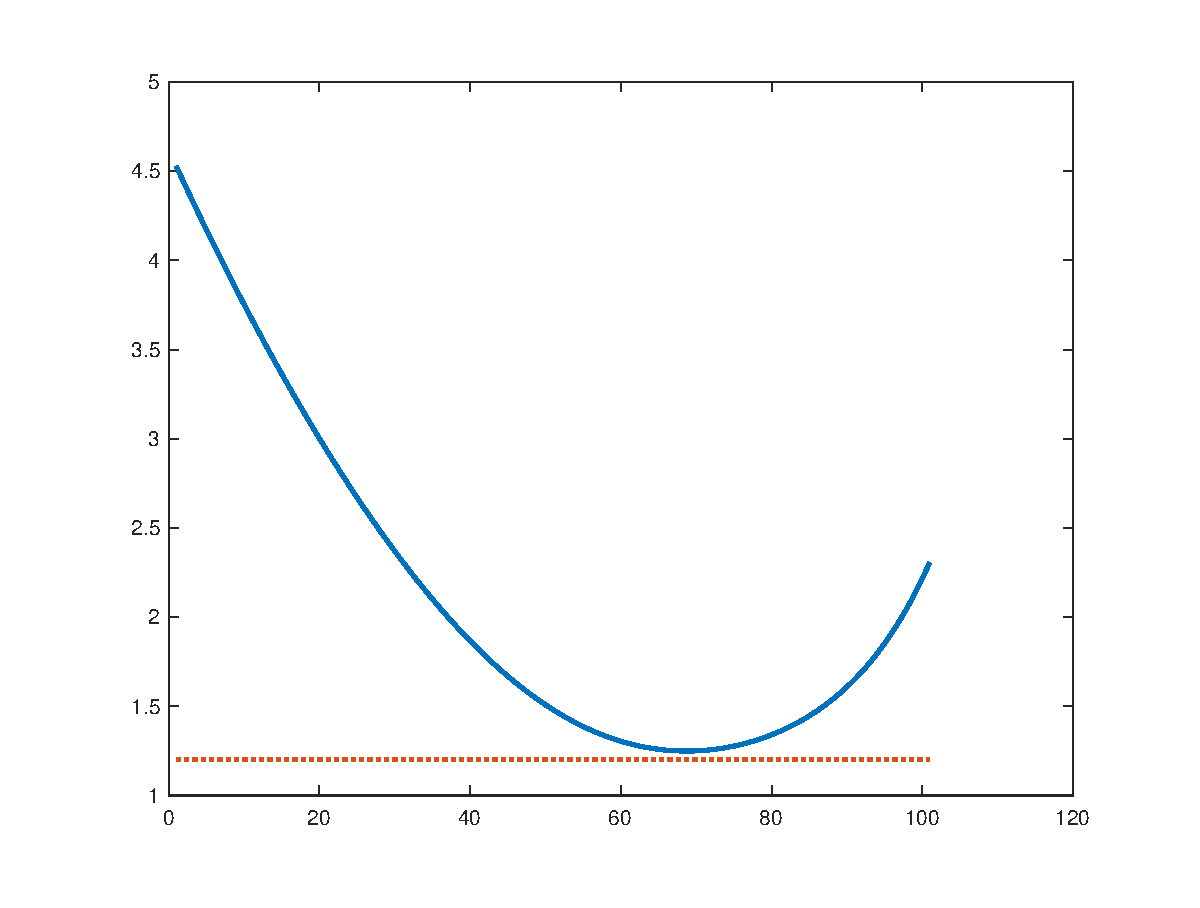
\includegraphics[width = 1.05\textwidth]{Figs/Chapter6/st_bezier_u_opt_distance_3d.eps}}
		\end{minipage}
	\end{center}
	\caption{Results of the proposed solution when used to optimise $\splinevar_i$ only.
    In the left image is depicted the same path as~\figref{FIG:ST-BEZIER-3D-INITIAL}, but with the new time behavior,
    normalized inside the interval $\lps 0,1 \rps$. The blue continuous line, in the right image, represents
    the new agent-obstacle distance, and the red dotted line is the fixed minimum safe distance.}%
    \label{FIG:ST-BEZIER-3D-U-RESULT}
\end{figure}
%%%%%%%%%%
%%%%%%%%%%
\begin{figure}[!t]
	\begin{center}
		\begin{minipage}{.45\linewidth}
			\centering
			\subfloat[]{%
				\label{FIG:ST-BEZIER-3D-PU-RESULT-A}%
				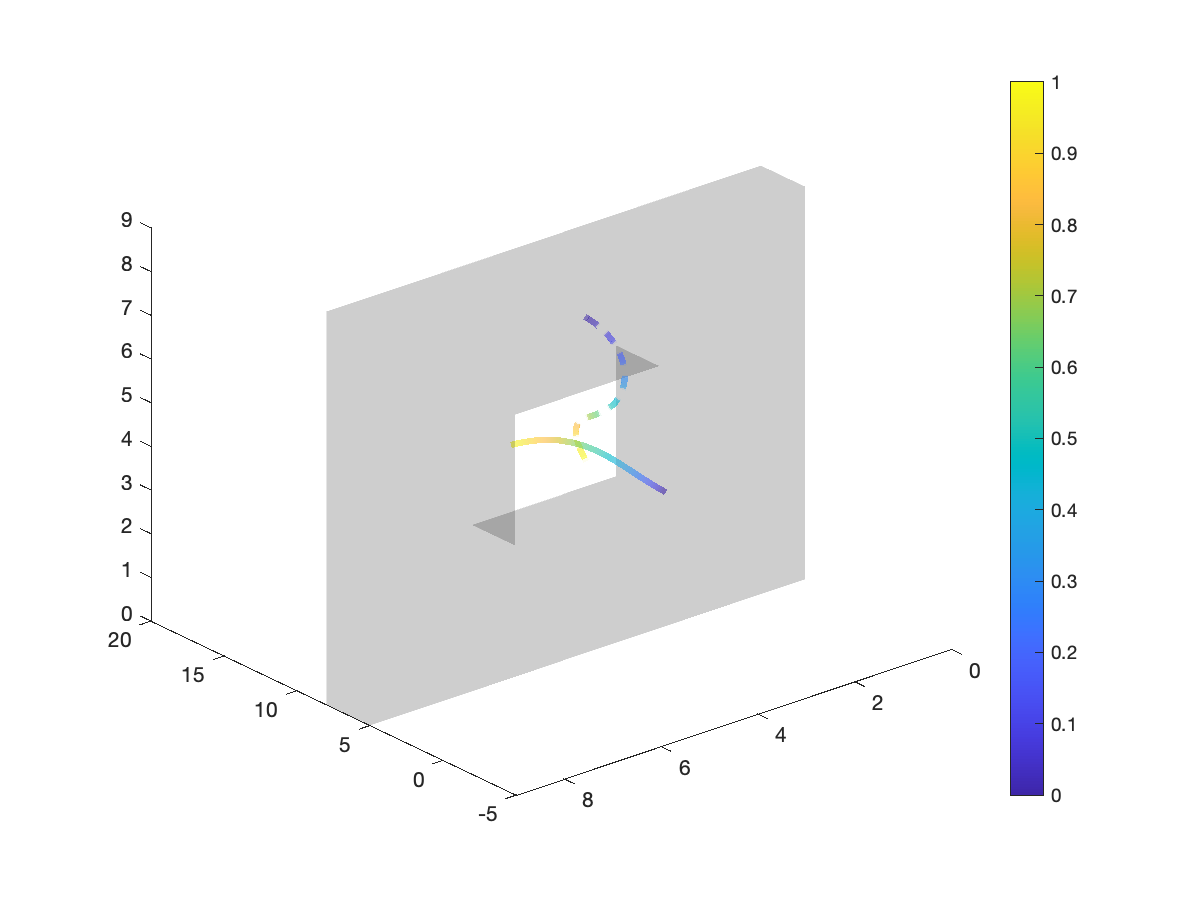
\includegraphics[width = 1.05\textwidth]{Figs/Chapter6/st_bezier_pu_opt_3d.eps}}
		\end{minipage}
		\begin{minipage}{.45\linewidth}
			\centering
			\subfloat[]{%
				\label{FIG:ST-BEZIER-3D-PU-RESULT-B}%
				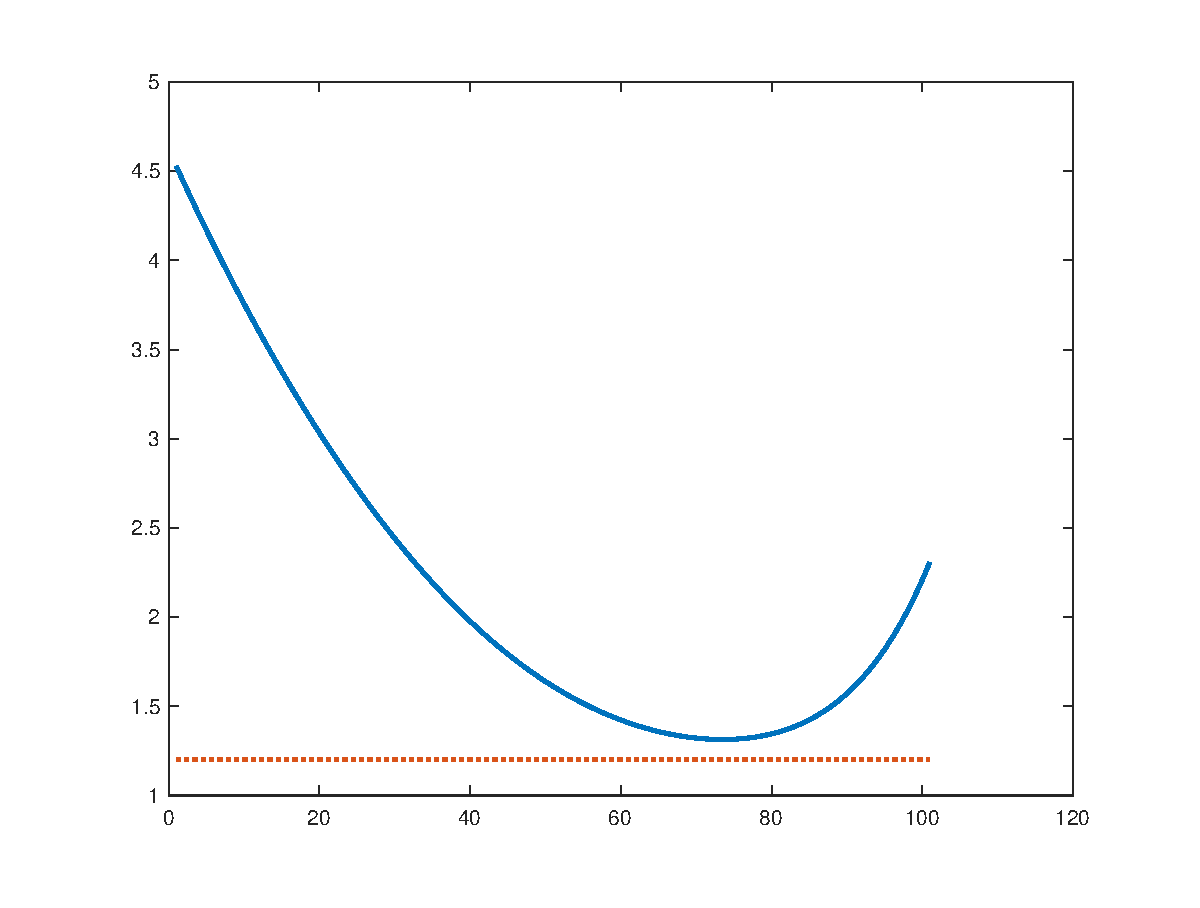
\includegraphics[width = 1.05\textwidth]{Figs/Chapter6/st_bezier_pu_opt_distance_3d.eps}}
		\end{minipage}
	\end{center}
	\caption{Results of the proposed solution when used to optimise both $\bs{\cpoint}_i$ and $\splinevar_i$.
    In the left image is depicted the new path with the new time behavior, normalized inside the interval $\lps 0,1 \rps$.
    The blue continuous line, in the right image, represents the new agent-obstacle distance, and the red dotted line is the
    fixed minimum safe distance.}%
    \label{FIG:ST-BEZIER-3D-PU-RESULT}
\end{figure}
%%%%%%%%%%
The proposed approach has been successfully applied in two different meaningful scenarios representing a two-dimensional
framework (\figref{FIG:ST-BEZIER-2D-INITIAL}), and a three-dimensional one (\figref{FIG:ST-BEZIER-3D-INITIAL}).
In both cases, the optimisation problem~\eqref{EQ:ST-SEPARATION-OPTIMISATION-PROBLEM} has been solved for $\splinevar_i$ only
and for both $\bs{\cpoint}_i$ and $\splinevar_i$. The obtained results are reported in Figures~\ref{FIG:ST-BEZIER-2D-U-RESULT}
and~\ref{FIG:ST-BEZIER-2D-PU-RESULT} for the two-dimensional case, and in Figures~\ref{FIG:ST-BEZIER-3D-U-RESULT}
and~\ref{FIG:ST-BEZIER-3D-PU-RESULT} for the three-dimensional one. In all figures the (a) image reports the resulting
trajectory along with its behavior in time, while image (b) depicts the agent-obstacle distance (blue line) with the fixed
minimum safe distance (red dotted line). In all simulations, we choose the loss function as in~\eqqref{EQ:ST-BEZIER-LOSS},
$d_{\text{safe}} = 0.25$, $v_{\text{max}} = 1.5m/s^2$, and $a_{\text{max}} = 0.5 m/s^2$.
The proposed solution succeeds, in each proposed scenario, to solve the trajectory replanning problem.
In the complete optimisation case, in Figures~\ref{FIG:ST-BEZIER-2D-PU-RESULT} and~\ref{FIG:ST-BEZIER-3D-PU-RESULT},
the algorithm is left free to trade-off between $\norm{\bs{\cpoint}_i - \bs{\cpoint}_i^j}$ and $\lb \splinevar_i - \splinevar_i^j \rb$
leading to a local optima with an higher final minimum distance.

%----------------------------------------------------------------------------------------
\section{Data-Driven Control Barrier Functions}
In this section, we detail a novel control-oriented approach to the replanning problem described in~\secref{SEC:REPLANNING-PROBLEM-DEFINITION},
focusing on the particular simplified case where only static obstacles may appear in a partially known environment.
The considered framework is well represented by~\eqqref{EQ:REPLANNING-OPTIMISATION-PROBLEM} with $\xset$ representing free and navigable
space, $\uset$ the set of all possible inputs, and $\xfun$ the considered system dynamics.
In this settings, the autonomous robot is pursuing an initial motion planned with only partial information about the surrounding
environment and concurrently is gathering information about it. The initial motion is then continuously refined with the collected
new information in order to ensure the robot safety at each time instant.
Motivated by this safety requirement, we ground the proposed solution on the notion of Control Barrier Function (CBF)~\cite{ames2016control}
which has been successfully demonstrated on many safety-critical applications~\cite{ames2016control, wang2017safe, hsu2015control}.
CBF applications ensure safety by enforcing the forward invariance of a \emph{safe set} described as a superlevel set of a candidate
function $\yfun$ which maps the system states to this notion of safety. In particular, the candidate function defines the hyper space
where the system is considered in a safe condition. Traditionally, these safety functions have been hand-designed. However,
depending on the application, designing such a candidate CBF is not straightforward in many practical settings. Consider, as an example,
the obstacle avoidance scenario, where the safe space is simply the free space, design the map $\yfun$ in this context requires
the complete environment knowledge, which is usually not completely a priori known.
Due to the aforementioned problem, we enforce the run-time adaptation of $\yfun$ via Gaussian process inference
exploiting real-time collected data, allowing for a constantly reshaping of the current motion with newly upcoming safe information.
The idea of learning the safe set from data is not new, in this sense Support Vector Machines (SVMs) were used in~\cite{srinivasan2020synthesis}
to parameterize CBFs with the help of sensor measurements. Neural networks were successfully used to regress the 
safety barrier function in~\cite{abate2020formal, zhao2020synthesizing, tsukamoto2020neural, gaby2021lyapunov}, while
a second-order cone program was formulated in~\cite{castaneda2021gaussian}, with GPs used for modeling the control input and the system uncertainties.
However, all these solutions are limited to offline training which limits their applicability in many practical scenarios.
Gaussian processes have been successfully used in~\cite{khan2021safety} and~\cite{khan2022gaussian} where the candidate function $\yfun$
is directly learned out of the collected data. The latter works, completely detach from a possible parameterised CBF and exploit the
GP regression in a completely data-driven scenario, without any a priori knowledge about the safe set.
However the quantity of collected data, required to build run-time the safe set, increases a lot with the system relative degree,
leading to poor, or even completely wrong, results.
Here we focused on the latter problem by formalising a new CBF-based solution that implements a Gaussian process regression 
requiring a limited number of samples whatever the system relative degree is. Then, the developed safety tool is successfully
implemented in the obstacle avoidance scenario.

We stress the fact that, unlike the approaches detailed in~\secref{SEC:REPLANNING-ALGORITHM} and~\secref{SEC:SPATION-TEMPORAL-SEPARATION},
the proposed solution does not require neither a resource consuming map building and maintenance, nor heavy 
random sampling procedure which may lead to very large set of samples, or possible trajectories, hard to handle.
The remain of this section unfolds as follow, in~\secref{SEC:CONTROL-BARRIER-FUNCTION} we briefly review key results on CBFs,~\secref{SEC:LEARNING-SAFE-SET}
describes a possible method to enforce the safe set learning, while in~\secref{SEC:PROPOSED-GAUSSIAN-CBF} and~\secref{SEC:CBF-RESULTS}
we formulate the proposed regulator and show the obtained results.

\subsection{Control Barrier Functions}%
\label{SEC:CONTROL-BARRIER-FUNCTION}
Consider the nonlinear control affine system
\begin{equation}%
    \label{EQ:CBF-INITIAL-SYSTEM}
    \begin{matrix}
        \dot{\xx} = \xfun \lp \xx \rp + \ufun \lp \xx \rp \uu, & \yy = \yfun \lp \xx \rp
    \end{matrix}
\end{equation}
where $\xx \in \R^{\dd{\xx}}$ is the system state, $\uu \in \uset \subset \R^{\dd{\uu}}$ is the input,
and $\yy \in \R^{\dd{\yy}}$ the measurable output. Moreover let $\xfun : \R^{\dd{\xx}} \mapsto \R^{\dd{\xx}}$
$\ufun : \R^{\dd{\xx}} \mapsto \R^{\dd{\xx} \times \dd{\uu}}$ and $\yfun : \R^{\dd{\xx}} \mapsto \R^{\dd{\yy}}$
Lipschitz continuous maps. Let the safety of~\eqref{EQ:CBF-INITIAL-SYSTEM} be encoded as the superlevel set
$\safeset$ of the smooth function $\yfun$
\begin{equation*}
    \safeset = \xset' = \left \{  \xx \in \R^{\dd{\xx}} : \yfun \lp \xx \rp \ge 0 \right \},
\end{equation*}
in this context we recall a couple of results from~\cite{xiao2019control, nguyen2016exponential, ames2016control}.
\begin{definition}%
    \label{DEF:CONTROL-BARRIER-FUNCTION}
    The map $\yfun \lp \xx \rp : \R^{\dd{\xx}} \mapsto \R^{\dd{\yy}}$ is defined as a Control Barrier Function (CBF),
    if there exists a class $\KK$ function $\alpha$, i.e. with the features (a) $\alpha \lp 0 \rp = 0$ and (b)
    $\alpha$ stricly increasing, such that the relation
    \begin{equation*}
        \sup_{\uu \in \uset} L_{\xfun} \yfun \lp \xx \rp + L_{\ufun} \yfun \lp \xx \rp \uu + \alpha \lp \yfun \lp \xx \rp\rp \ge 0,
    \end{equation*}
    holds for any $\xx \in \safeset$.
\end{definition}
In the previous definition the quantities $L_{\xfun} \yfun \lp \xx \rp$ and $L_{\ufun} \yfun \lp \xx \rp$ are the directional derivatives
of $\yfun$, along the flow defined by $\xfun$ and $\ufun$, respectively (along the literature called \emph{Lie derivatives}).
With the aforementioned definition at hand, we can easily enforce the system safety, which in this context implies no collisions,
by shaping the control input $\uu$ of~\eqref{EQ:CBF-INITIAL-SYSTEM} over the designed CBF in~\defref{DEF:CONTROL-BARRIER-FUNCTION}.
\begin{theorem}%
    \label{TH:SAFE-INVARIANCE}
    Given a nonlinear system as in~\eqqref{EQ:CBF-INITIAL-SYSTEM}, with a defined safe set $\safeset \subset \R^{\dd{\xx}}$,
    and a smooth control barrier function $\yfun \lp \xx \rp : \R^{\dd{\xx}} \mapsto \R^{\dd{\yy}}$, any Lipschitz continuous
    control law $\uu \lp t \rp \in \R^{\dd{\uu}}$ satisfying
    \begin{equation}%
        \label{EQ:CBF}
        L_{\xfun} \yfun \lp \xx \lp t \rp\rp + L_{\ufun} \yfun \lp \xx \lp t \rp\rp \uu \lp t \rp + \alpha \lp \yfun \lp \xx \lp t \rp\rp\rp \ge 0,
    \end{equation}
    for any $\xx \in \R^{\dd{\xx}}$, makes the safe set $\safeset$ forward invariant for~\eqref{EQ:CBF-INITIAL-SYSTEM}.
\end{theorem}
The reader can immediately conceive from~\thref{TH:SAFE-INVARIANCE} and~\defref{DEF:CONTROL-BARRIER-FUNCTION} the very limiting
requirement to have relative degree (here referred to as $\order$) equal to one, $\order = 1$.
For systems with $\order > 1$, we require an extension to the CBF notion defined so far. In particular, referring
to~\cite{nguyen2016exponential, xiao2019control}, let's introduce the concept of Exponential Control Barrier Function (ECBF).
\begin{definition}
    The smooth function $\yfun \lp \xx \rp: \R^{\dd{\xx}} \mapsto \R^{\dd{\yy}}$, with relative degree $\order$, is defined as an
    exponential control barrier function, if there exists a set of coefficients $ \Lambda \in \R^{\order}$ such that for any $\xx \in \R^{\dd{\xx}}$
    \begin{equation}%
        \label{EQ:ECBF}
        \sup_{\uu \in \uset} L^{\order}_{\xfun} \yfun \lp \xx \rp + L_{\ufun}L_{\xfun}^{\order-1} \yfun \lp \xx \rp \uu + \Lambda\T \HH \ge 0
    \end{equation}
    holds with $\HH = \lps \yfun \lp \xx \rp, L_{\xfun} \yfun \lp \xx \rp, \dots, L^{\order-1}_{\xfun} \yfun \lp \xx \rp\rps\T \in \R^{\order}$
    the Lie derivative vector for $\yfun$, and $\Lambda = \lps \lambda_0, \lambda_1, \dots, \lambda_{\order-1} \rps\T$ is a
    coefficient gain vector for $\HH$ which can be conputed via standard linear control techniques.
\end{definition}
The functions~\eqref{EQ:CBF} or~\eqref{EQ:ECBF} can then be combined with Quadratic Programs (QPs) to achieve safety constrained control,
in particular, for high relative degree systems, the forward invariance of the safe set $\safeset = \{ \xx \in \R^{\dd{\xx}} : \yfun \lp \xx \rp \ge 0\}$
can be enforced solving the following optimisation problem
\begin{equation}%
    \label{EQ:CBF-OPTIMISATION-PROBLEM}
    \begin{split}
        \uu = \arg \min_{v \in \uset} & \frac{1}{2} \norm{v - \uu\s} \\
        \text{subj. to} \hspace{0.2cm} & L_{\xfun}^{\order} \yfun \lp \xx \rp + L_{\ufun} L_{\xfun}^{\order-1} \yfun \lp \xx \rp v + \Lambda\T\HH \ge 0
    \end{split}
\end{equation}
with $\uu\s \in \R^{\dd{\uu}}$ previous planned control input, referred to as \emph{nominal input}.
\begin{remark}
    The problem~\eqref{EQ:CBF-OPTIMISATION-PROBLEM} resembles the replanning problem~\eqref{EQ:REPLANNING-OPTIMISATION-PROBLEM}
    borrowing the same loss and with the safe and dynamic constraints condensed in~\eqqref{EQ:ECBF}.
\end{remark}

\subsection{Learning the Safe Set}%
\label{SEC:LEARNING-SAFE-SET}
The major issue in using CBF to enforce safety lies in designing the candidate function $\yfun$, whose superlevel set
must encode all safe regions where the system state is allowed to evolve.
This problem is mainly present also in obstacle avoidance scenarios where the environment in not a priori known
making impossible the design of $\yfun$. To overcome this limitation,~\cite{khan2022gaussian} proposes to handle
the construction of $\yfun$ following a complete data-driven approach: the key idea was to model this unknown map
as a realisation of a Gaussian process. In particular, supposing to have access to a data-set
$\lp \bs{\xx}, \bs{\yy} \rp = \{ \lp \xx(t_1), \yy(t_1) \rp, \dots, \lp \xx(t_{N}), \yy(t_{N}) \rp \}$
of $N$ samples, with each pair $(\xx(t_h),$ $ \yy(t_h)) \in \R^{\dd{\xx}} \times \R^{\dd{\yy}}$ obtained as
$\yy(t_h) = \yfun \lp \xx(t_h) \rp + \noise(t_h)$ with $\noise(t_h) \sim \NN \lp 0, \nn I_{\dd{\yy}}\rp$
be a white Gaussian noise, then an approximation of $\yfun$ can be computed as
\begin{equation}%
   \label{EQ:CBF-GAUSSIAN-REGRESSION}
   \begin{split}
      \pmu \lp \xx \rp & = \kv \lp \xx \rp\T \lp\km + \nn I_{N}\rp^{-1}\bs{\yy}, \\
      \pvar \lp \xx \rp & = \kf \lp \xx, \xx \rp - \kv \lp \xx \rp \T \lp\km + \nn I_{N}\rp^{-1}\kv \lp \xx \rp,
   \end{split}
\end{equation}
where $\km \in \R^{N \times N}$ is the \textit{Gram matrix} whose $(k,h)$th entry is $\km_{k,h} = \kf \lp \bs{\xx}_k, \bs{\xx}_h \rp$,
with $\bs{\xx}_k$ the $k$th entry of $\bs{\xx}$, $\kv \lp \xx \rp \in \R^{N}$ is the kernel vector whose $k$th component is
$\kv_k \lp \xx \rp = \kf \lp \xx, \bs{\xx} \rp$, and $\kf \lp \xx, \xx' \rp$ is a custom kernel function~\cite{rasmussen2003gaussian}.
For further information about Gaussian regression and about the kernel structure the reader is referred to~\appref{SEC:GAUSSIAN-PROCESS-APPENDIX}.
Gaussian regression works by iteratively restricting the pool of possible functions, conditioning a prior Gaussian distribution on the
collected dataset. In this sense,~\eqqref{EQ:CBF-GAUSSIAN-REGRESSION} expresses the a posteriori mean ($\pmu$) and variance ($\pvar$)
computed after the collection of $N$ samples $\lp \bs{\xx}, \bs{\yy} \rp$.
In this context, the computed mean represents the ``best'' function approximation, while $\pvar$ quantifies the amount of uncertainties
affecting the current estimation, as it strongly depends on the amount of data collected near the evaluating point $\xx$.
Although the estimation $\pmu$ of $\yfun$ can be directly used inside the optimisation problem~\eqref{EQ:CBF-OPTIMISATION-PROBLEM}
in place of $\yfun$, we should be careful of possible errors and uncertainties in the reconstructed approximation as a wrong value of
$\pmu$ may make condition~\eqref{EQ:ECBF} holds even in unsafe conditions.
As a matter of fact, evaluating an unknown function out of data may lead to wrong results, especially if the collected data are
poorly informative or very scattered.
To overtake this particular problem,~\cite{khan2022gaussian} proposed a re-reading of the candidate function keeping into consideration
also the provided a posteriori variance of the current estimation $\pmu$, thus $\yfun$ has been reformulated as
\begin{equation*}
    h_{\text{GP}}\lp \xx \rp = \pmu \lp \xx \rp - \rho \pvar \lp \xx \rp,
\end{equation*}
with $\rho \in \R^{+}$ a tunable value, leading to the new optimisation problem
\begin{equation*}
    \begin{split}
        \uu = & \arg \min_{v \in \uset} \frac{1}{2} \norm{v - \uu\s} \\
        & \text{s.t.} \hspace*{0.2cm} L_{\xfun}^{\order} \yfun_{\text{GP}}\lp \xx \rp +
                                      L_{\ufun} L_{\xfun}^{\order-1} \yfun_{\text{GP}} \lp \xx \rp v + \Lambda\T\HH \ge 0.
    \end{split}
\end{equation*}
The aforementioned approach is very promising under the perspective of adapt CBF tools to a very large number of use cases, especially
when an analytical formulation of $\yfun$ is not accessible, but results to be very poor practically when dealing with systems with
high relative degrees $\order > 1$ because of loss of information during Gaussian process differentiation~\cite{holsclaw2013gaussian}.
Furthermore, the parameter $\rho$ results to be the key to obtain good performances even with $\order = 1$, thus a very careful tuning
is required to make the algorithm works correctly.
The aforementioned problems motivated our research in the field of Gaussian control barrier functions toward more general and resilient
solutions, especially tailored for high relative degree systems.

\subsection{Proposed Gaussian Control Barrier Function}%
\label{SEC:PROPOSED-GAUSSIAN-CBF}
%%%%%%%%%%
\begin{figure}[!t]
	\begin{center}
		\begin{minipage}{.45\linewidth}
			\centering
			\subfloat[]{%
				\label{FIG:CBF-RESULTS-COMPARISON-A}%
				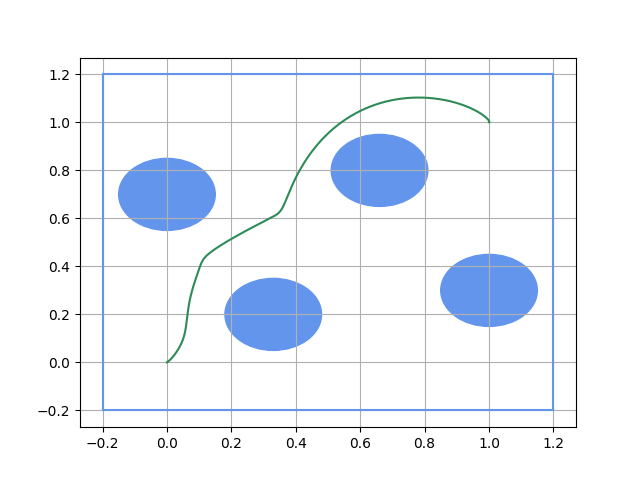
\includegraphics[width = 1.05\textwidth]{Figs/Chapter6/cbf_0505.png}}
		\end{minipage}
		\begin{minipage}{.45\linewidth}
			\centering
			\subfloat[]{%
				\label{FIG:CBF-RESULTS-COMPARISON-B}%
				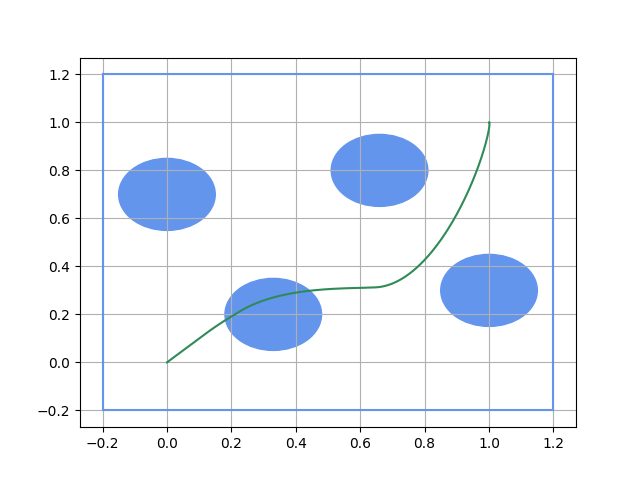
\includegraphics[width = 1.05\textwidth]{Figs/Chapter6/cbf_0505_gp.png}}
		\end{minipage}
		\begin{minipage}{.45\linewidth}
			\centering
			\subfloat[]{%
				\label{FIG:CBF-RESULTS-COMPARISON-C}%
				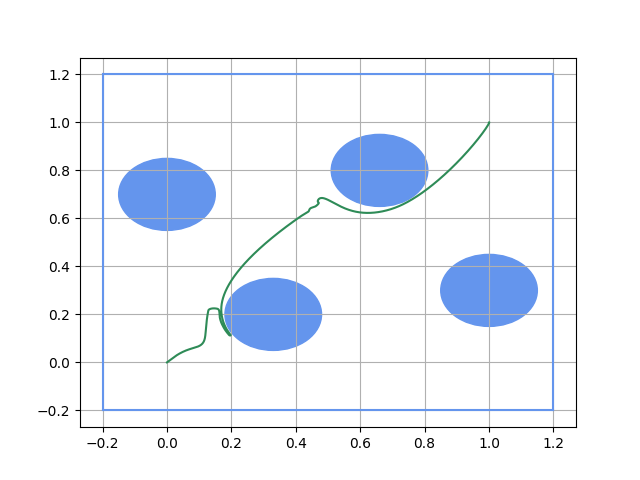
\includegraphics[width = 1.05\textwidth]{Figs/Chapter6/cbf_0505_gp_hg.png}}
		\end{minipage}
	\end{center}
	\caption{Comparison between (a) classic ECBF, (b) GP-CBF proposed by~\cite{khan2022gaussian}, and (c) GP-CBF proposed here.
    In image (a) the safe set is designed using the complete knowledge of the environment, while in images (b) and (c) the
    candidate function is reconstructed run-time using the collected sensor data.}%
    \label{FIG:CBF-RESULTS-COMPARISON}
\end{figure}
%%%%%%%%%%
The proposed regulator reads as
\begin{equation}%
    \label{EQ:CBF-PROPOSED-OBSERVER}
    \dot{\zz} = A\zz + B \lp L_{\xfun} \pmu \lp \xx \rp + L_{\ufun} \pmu \lp \xx \rp \uu \rp + G \lp l \rp H \lp \yy - C\zz \rp,
\end{equation}
with output
\begin{equation}%
    \label{EQ:CBF-PROPOSED-OPTIMISATION-PROBLEM}
    \begin{split}
        \uu = \arg \min_{v \in \uset} & \frac{1}{2} \norm{v - \uu\s} + L_{\ufun} \pvar \lp \xx \rp v \\
        \text{subj. to} \hspace{0.2cm} & L_{\xfun} \pmu \lp \xx \rp + L_{\ufun} \pmu \lp \xx \rp v + \Lambda\T\HH \ge 0.
    \end{split}
\end{equation}
As emerges from~\eqqref{EQ:CBF-PROPOSED-OBSERVER}, the proposed regulator consists in a standard high-gain observer
with $A$, $B$, and $C$ matrices in prime form
\begin{equation*}
    \begin{matrix}
        A =
        \begin{pmatrix}
            0_{(\order-1)\dd{\yy} \times \dd{\yy}} & I_{(\order-1)\dd{\yy}} \\
            0_{\dd{\yy} \times \dd{\yy}} & 0_{\dd{\yy} \times (\order-1)\dd{\yy}}
        \end{pmatrix}, &
        B =
        \begin{pmatrix}
            0_{(\order-1)\dd{\yy} \times \dd{\yy}} \\
            I_{\dd{\yy}}
        \end{pmatrix},
    \end{matrix}
    \end{equation*}
    \begin{equation*}
    C =
    \begin{pmatrix}
        I_{\dd{\yy}} & 0_{\dd{\yy} \times (\order-1)\dd{\yy}}
    \end{pmatrix},
\end{equation*}
and $G(l) = \text{diag} \lp l I_{\dd{\yy}}, l^{2} I_{\dd{\yy}}, \dots, l^{r} I_{\dd{\yy}} \rp$,
$H = \text{diag} \lp H_1, \dots, H_r \rp$, and $H_i = \text{diag} \big( h^1_i, \dots$ $\dots, h^{\dd{\yy}}_i \big)$ with
$\{h_{1}^j, h_{2}^j, \dots, h_{r+1}^j\}$ for all $j = 1, \dots, \dd{\yy}$ coefficients of a Hurwitz polinomial,
where $l \in \R_{>0}$ is a control parameter.
In this context, the proposed observer is meant to directly reconstruct $L_{\xfun}^{\order-1} \yfun$, that in turn is
feeded back to a Gaussian regressor which outputs an analytical and differentiable estimate
\begin{equation*}
	\pmu \lp \xx \rp = \kv \lp \xx \rp\T \lps \km + \nn I_N \rps^{-1} \bs{\zz},
\end{equation*}
with $\bs{\zz}$ extracted from the recostructed data-set
\begin{equation*}
    \lp \bs{\xx}, \bs{\zz} \rp = \{ \lp \xx(t_1), \zz_{\order-1}(t_1) \rp, \dots, \lp \xx(t_{N}), \zz_{\order-1}(t_{N}) \rp \}.
\end{equation*}
The regressed directional derivate is then used to reconstruct the observer consistency term~\cite{buisson2021joint}.
Equation~\eqref{EQ:CBF-PROPOSED-OPTIMISATION-PROBLEM} reformulates the one-relative-degree problem~\eqref{EQ:CBF-OPTIMISATION-PROBLEM}
in this particular framework. Note that the used candidate function does not take into account any uncertainties in the
retrieved estimation, which in turn are encode inside the loss function as $L_{\ufun} \pvar \lp \xx \rp v$, with
$\pvar$ the a posteriori Gaussian variance
\begin{equation*}
	\pvar \lp \xx \rp = \kf \lp \xx,\xx \rp - \kv \lp \xx \rp\T \lps \km + \nn I_N \rps^{-1} \kv \lp \xx \rp.
\end{equation*}
\begin{remark}
    Although the new loss proposed in~\eqqref{EQ:CBF-PROPOSED-OPTIMISATION-PROBLEM} presents a slightly different structure
    with respect to classical CBF formulation~\eqref{EQ:CBF-OPTIMISATION-PROBLEM} and with respect to the formulated
    problem in~\secref{SEC:REPLANNING-PROBLEM-DEFINITION}, it still succeed in solving the obstacle avoidance problem as the
    collision is encoded as optimisation hard constraint. Moreover, minimise $L_{\ufun} \pvar \lp \xx \rp v$ directly
    implies a minimisation of the induced uncertainties affecting $\pmu$ as the agent is forced to navigate toward already
    visited frontiers. As a matter of fact, the aforementioned term comes out from~\eqqref{EQ:ECBF} cosidering
    $\yfun = \pmu + \pvar$
    \begin{equation*}
        \sup_{\uu \in \uset} L_{\xfun} \yfun \lp \xx \rp + L_{\ufun} \yfun \lp \xx \rp v + \Lambda\T\HH \ge 0,
    \end{equation*}
    \begin{equation*}
        L_{\xfun} \lp \pmu \lp \xx \rp + \pvar \lp \xx \rp \rp + L_{\ufun} \lp \pmu \lp \xx \rp + \pvar \lp \xx \rp \rp v.
    \end{equation*}
    We stress the fact that encoding an uncertainties term inside the cost formulation drops the necessity to introduce a weight $\rho$
    inside the candidate function, as done in~\cite{khan2022gaussian}, whose wrong tuning may degrade the algorithm performance.
\end{remark}
\begin{remark}
    The proposed solution~\eqref{EQ:CBF-PROPOSED-OBSERVER}-\eqref{EQ:CBF-PROPOSED-OPTIMISATION-PROBLEM} is well suited for
    high relative degree applications as the regressed map $\pmu$ is differentiated only once, leading to a very few loss of
    information. In the context of Gaussian process, the latter property implies the possibility to keep the value of $N$ low,
    leading to light real-time training procedures.
\end{remark}
We conclude this section by recalling two basic properties which the regressor should undergo to make the proposed solution works 
correctly. We stress the fact that the assumptions reported below are not restrictive under the practical point of view, and can be
easily satisfied by all commonly used kernels. The following assumptions are borrowed from~\cite{buisson2021joint}.
\begin{assumption}%
    $\pmu$ is Lipschitz continuous with Lipschitz constant $L_{\pmu}$, and its norm is bounded by $\pmu_{\text{max}}$.
 \end{assumption}
 \begin{assumption}%
    The kernel function $\kf(\cdot, \cdot)$ is Lipschitz continuous with constant $L_{\kf}$, with a locally Lipschitz derivative of constant $L_{d\kf}$,
    and its norm is bounded by $\kf_{\text{max}}$.
 \end{assumption}

\subsection{Experimental Results}%
\label{SEC:CBF-RESULTS}
%%%%%%%%%%
\begin{figure}[!t]
	\begin{center}
		\begin{minipage}{.45\linewidth}
			\centering
			\subfloat[]{%
				\label{FIG:CBF-RESULTS-FAIL-A}%
				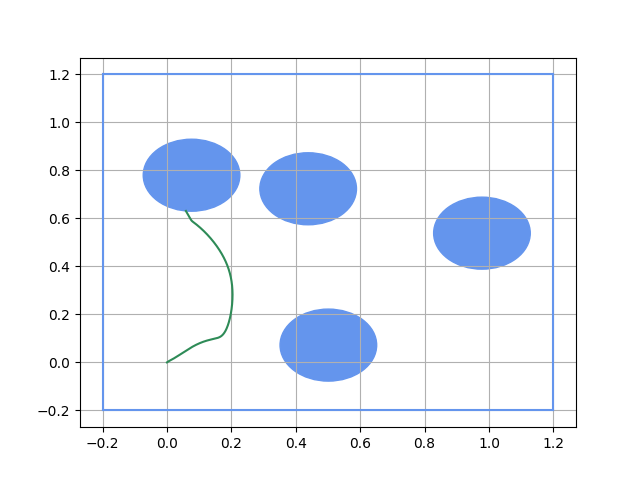
\includegraphics[width = 1.05\textwidth]{Figs/Chapter6/cbf_0505_gp_hg_test_1.png}}
		\end{minipage}
		\begin{minipage}{.45\linewidth}
			\centering
			\subfloat[]{%
				\label{FIG:CBF-RESULTS-FAIL-B}%
				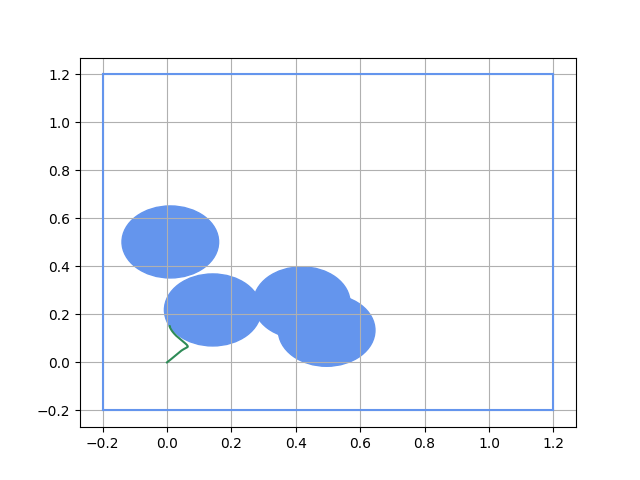
\includegraphics[width = 1.05\textwidth]{Figs/Chapter6/cbf_0505_gp_hg_test_2.png}}
		\end{minipage}
	\end{center}
	\caption{Results obtained in challenging environments when applying the proposed approach without
    taking into account estimation uncertainties carried by $\pvar$. As the reader can observe, the proposed solution
    does not make the agent colliding, but can stuck it close to obstacles.}%
    \label{FIG:CBF-RESULTS-FAIL}
\end{figure}
%%%%%%%%%%
%%%%%%%%%%
\begin{figure}[!t]
	\begin{center}
		\begin{minipage}{.45\linewidth}
			\centering
			\subfloat[]{%
				\label{FIG:CBF-RESULTS-WIN-A}%
				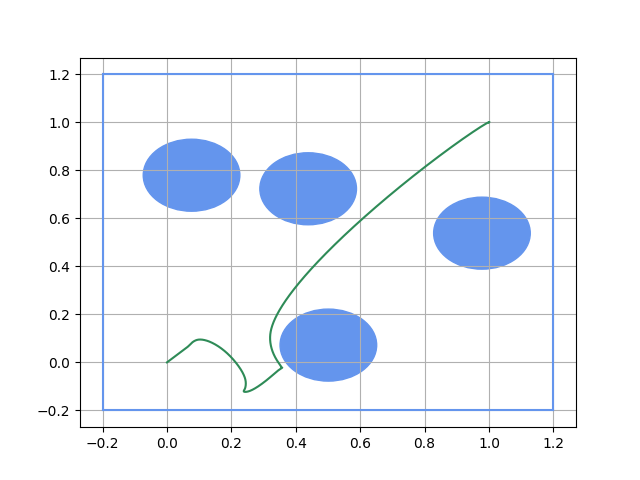
\includegraphics[width = 1.05\textwidth]{Figs/Chapter6/cbf_0505_gp_hg_norm_test_1.png}}
		\end{minipage}
		\begin{minipage}{.45\linewidth}
			\centering
			\subfloat[]{%
				\label{FIG:CBF-RESULTS-WIN-B}%
				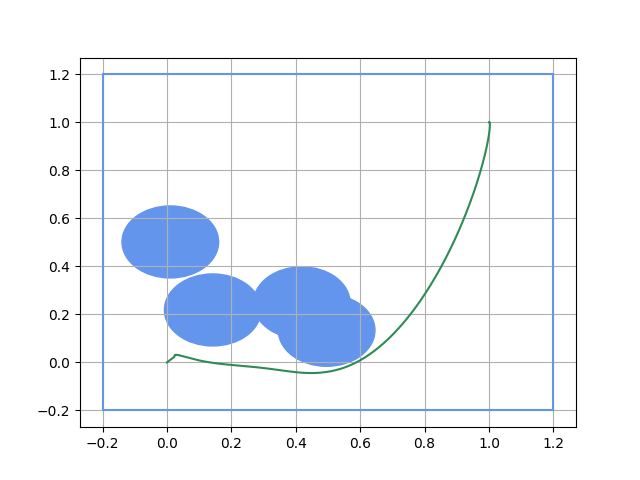
\includegraphics[width = 1.05\textwidth]{Figs/Chapter6/cbf_0505_gp_hg_norm_test_2.png}}
		\end{minipage}
	\end{center}
	\caption{Results obtained in challenging environments when applying the overall proposed approach.
    The encoded uncertainties via $\pvar$ drive the agent in regions with low uncertainties, making the final solution
    working in all cases.}%
    \label{FIG:CBF-RESULTS-WIN}
\end{figure}
%%%%%%%%%%
The proposed approach has been applied to a synthetic scenario and tested against the classical ECBF, where the safe
set design has been made using the full knowledge about the navigating environment, and the state-of-the-art
Gaussian-based CBF proposed by~\cite{khan2022gaussian}. In both the learning techniques, the training data are collected
real time, while the agent is moving inside the environment.
The testing scenario (see~\figref{FIG:CBF-RESULTS-COMPARISON}) is equal in all experiments and consists of four shpere-like
obstacles with random positions and four surrounding walls. The agent is modeled a simple double integrator with acceleration
as control input, while the nominal control input $\uu\s$ consists in a straight line from the initial to the goal position.
In this settings, the candidate function $\yfun$ is modeled as the distance from the closest obstacle, following the
Euclidean Signed Distance Field (ESDF) principle~\cite{oleynikova2017voxblox}.
The obtained results are reported in Figures~\ref{FIG:CBF-RESULTS-COMPARISON},~\ref{FIG:CBF-RESULTS-FAIL}, and~\ref{FIG:CBF-RESULTS-WIN}.
In particular,~\figref{FIG:CBF-RESULTS-COMPARISON} depicts a comparison between the classical ECBF, the GP-CBF proposed by~\cite{khan2022gaussian},
and our approach when applied in the same settings described above. The classical ECBF, designed on the complete knowledge of the
environment, always succeeds in safely steering the agent to the goal and its results are kept here as a baseline to follow in the case
where no prior information about the obstacles is provided. As the reader can see, from~\figref{FIG:CBF-RESULTS-COMPARISON},
the approach proposed by~\cite{khan2022gaussian} sometimes fails, especially in highly cluttered environment, while our approach
always wins. To highlight the fundamental role which plays the regulariser $L_{\ufun} \pvar \lp \xx \rp v$
in~\eqref{EQ:CBF-PROPOSED-OPTIMISATION-PROBLEM}, we reported here two simulations in Figures~\ref{FIG:CBF-RESULTS-FAIL} and~\ref{FIG:CBF-RESULTS-WIN}
where the proposed approach is applied without and with the regularisation term. In particular, in~\figref{FIG:CBF-RESULTS-FAIL}
the term is not present, while in~\figref{FIG:CBF-RESULTS-WIN} the optimisation problem is solved with the proposed complete loss function.
It is worth to remark how in both cases the agent does not collide with obstacles, but in the first reported simulations the high uncertainties
affecting the estimated candidate function made the agent stuck near to obstacles.

%----------------------------------------------------------------------------------------
\section{Contributions}
In this chapter we reviewed and discussed the problem of real-time trajectory replanning in front of new environmental information.
The chapter develops firstly by reviewing a state-of-the-art solution to the problem at hand, adapted, re-implemented and tested in the
specific case of the Leonardo drone contest. The selected solution performed well and succeed in replanning jerk-continuous trajectories
well suited for quadcopter navigation. Then, two novel solutions have been described and analyzed, one primarily focused on the specific
case of moving obstacles and multi-agent scenarios, and the second one focused on static environments.
The proposed flow embraces a research direction especially focused on numeric and system theory-oriented solutions where the possibility
of success can be easily assessed via analysis tools commonly used in the system theory field.
As a future research direction, we will continue to follow this idea and try to encode Lyapunov theory in novel trajectory
plaNning, or replanning, techniques yielding to very high reliable and robust solutions.

%------------------------------------------------